
\documentclass{article}

\usepackage{graphicx}
\usepackage{amsmath}
\usepackage{placeins}

\usepackage[margin=1in]{geometry}
\usepackage{float}


\def\hwtitle{Computational Physics HW3}
\def\hwauthor{Ethan Rooney}
\def\hwdate{2020-02-12}

\usepackage{fancyhdr}
\lhead{\hwauthor}
\chead{\hwtitle}
\rhead{\hwdate}
\lfoot{\hwauthor}
\cfoot{}
\rfoot{\thepage}
\renewcommand{\footrulewidth}{0.4pt}
\pagestyle{fancy}

\author{\hwauthor}
\title{\hwtitle}
\date{\hwdate}

\begin{document}

\maketitle
\thispagestyle{fancy}

\section{Introduction}
 
This weeks homework is the continuation of Week 3. We are extending and generalizing from 2 body interactions to $n$-body systems. The math is essentially unchanged from last weeks assignment. We are utilizing the RK2 integrator, with more bodies.

\section{Results}

\subsection{Question 0}

Here we check the validity of our generalized RK2 integrator with a 2 body problem. A "earth-like" object is put into motion 1 AU away from a "sun-like" object with the same velocity as the earth. We see a circular orbit. This is a good start.

\begin{figure}[!htb]
	\begin{center}
		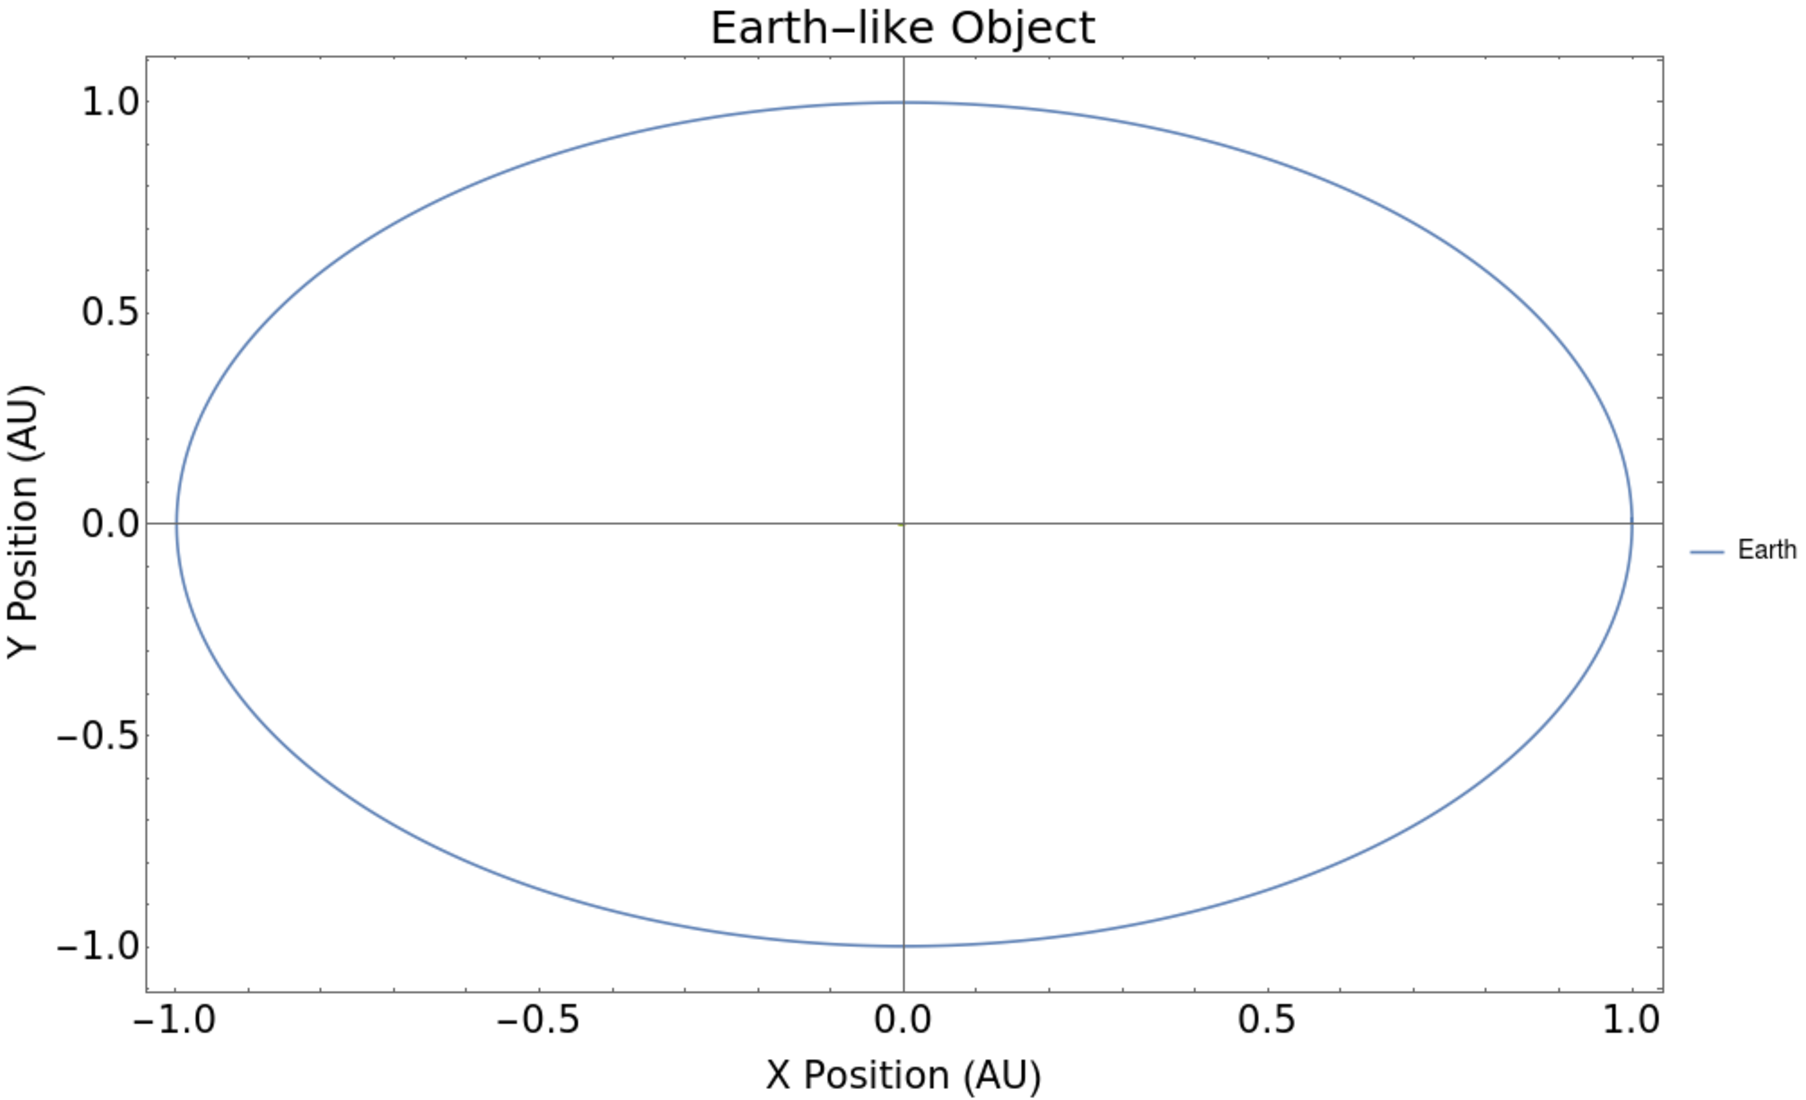
\includegraphics[width=0.5\textwidth]{p0.pdf}
	\end{center}
	\caption{}
\label{fig:qual}
\end{figure}
\FloatBarrier

\subsection{Question 1}

We continue the extension of last weeks work with a trial run of a 3-body system much like the one we find in our own solar system.

\subsubsection{1}

The Moon's orbit is close enough to Earth's that the orbit of Earth is obscured.

\begin{figure}[!htb]
	\begin{center}
		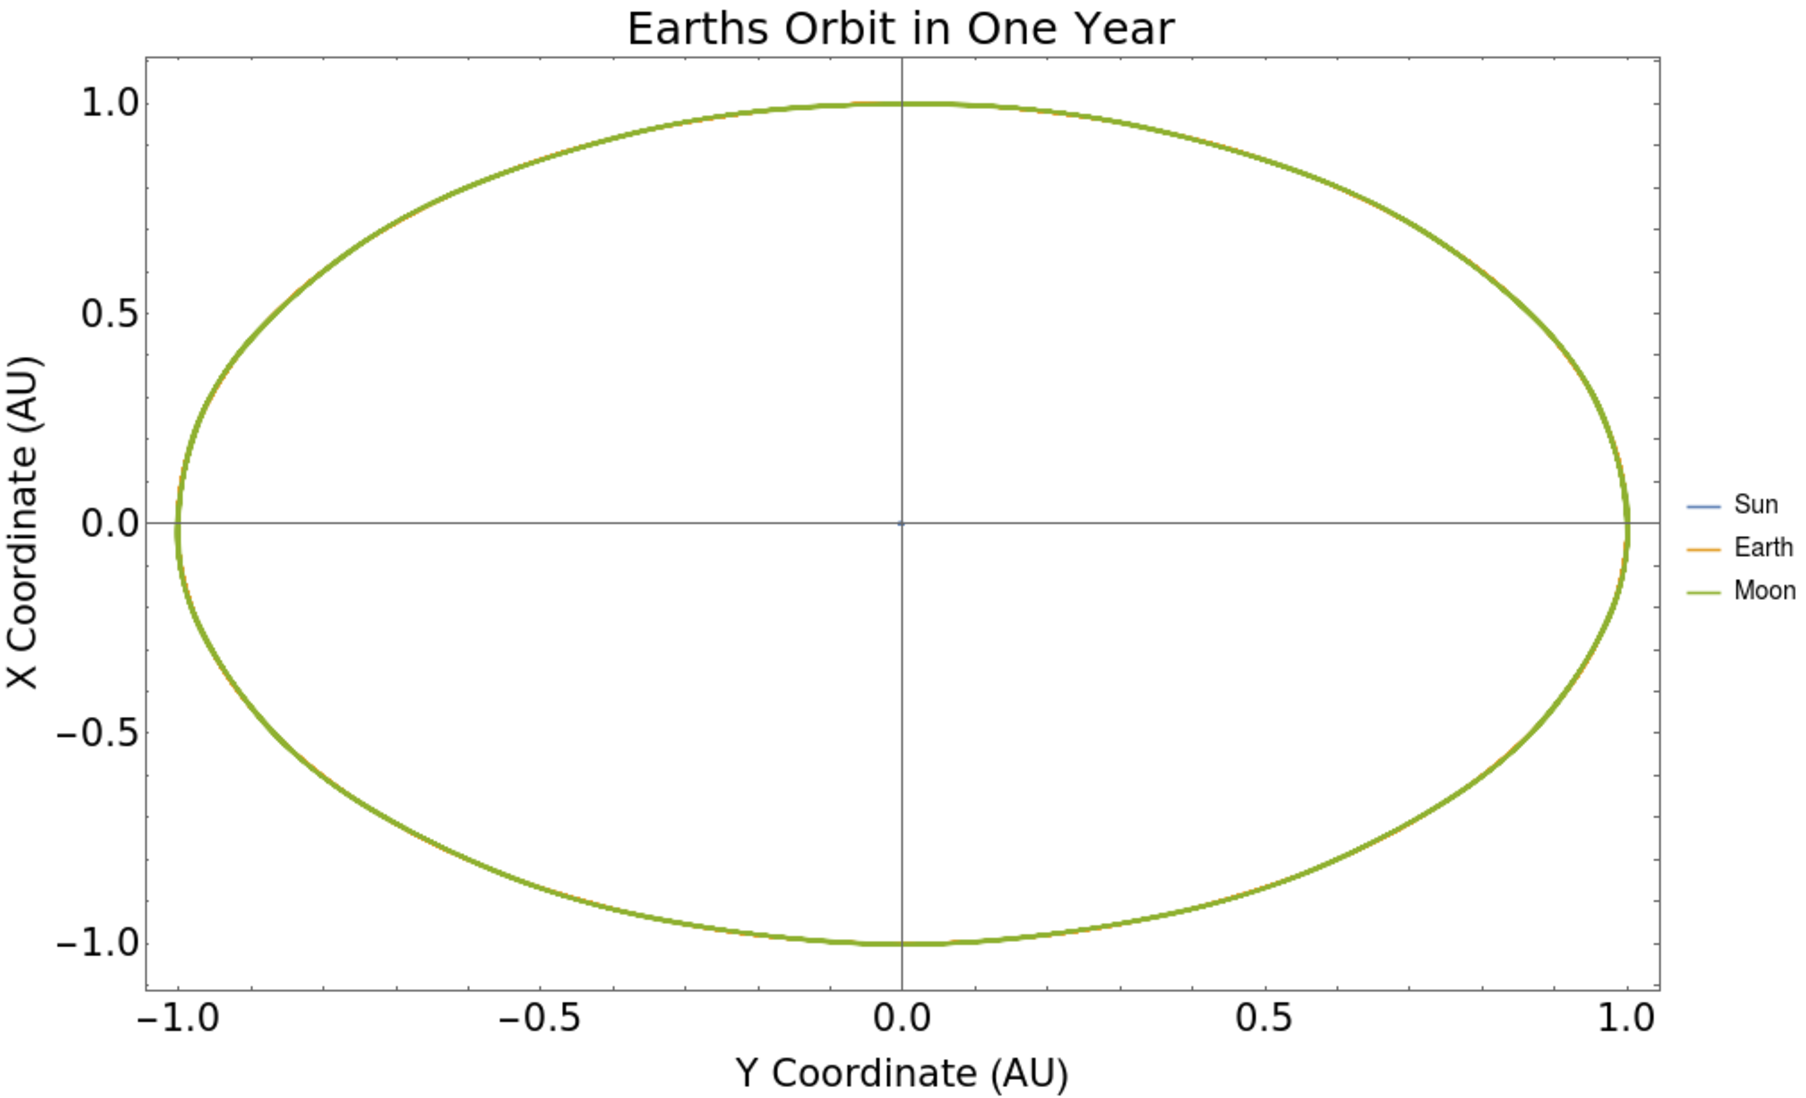
\includegraphics[width=0.5\textwidth]{p1-1a.pdf}
	\end{center}
	\caption{}
\label{fig:qual}
\end{figure}
\FloatBarrier

Over 8 Years the Moon slowly drifts towards, and away from the earth with a net movement away.

\begin{figure}[!htb]
	\begin{center}
		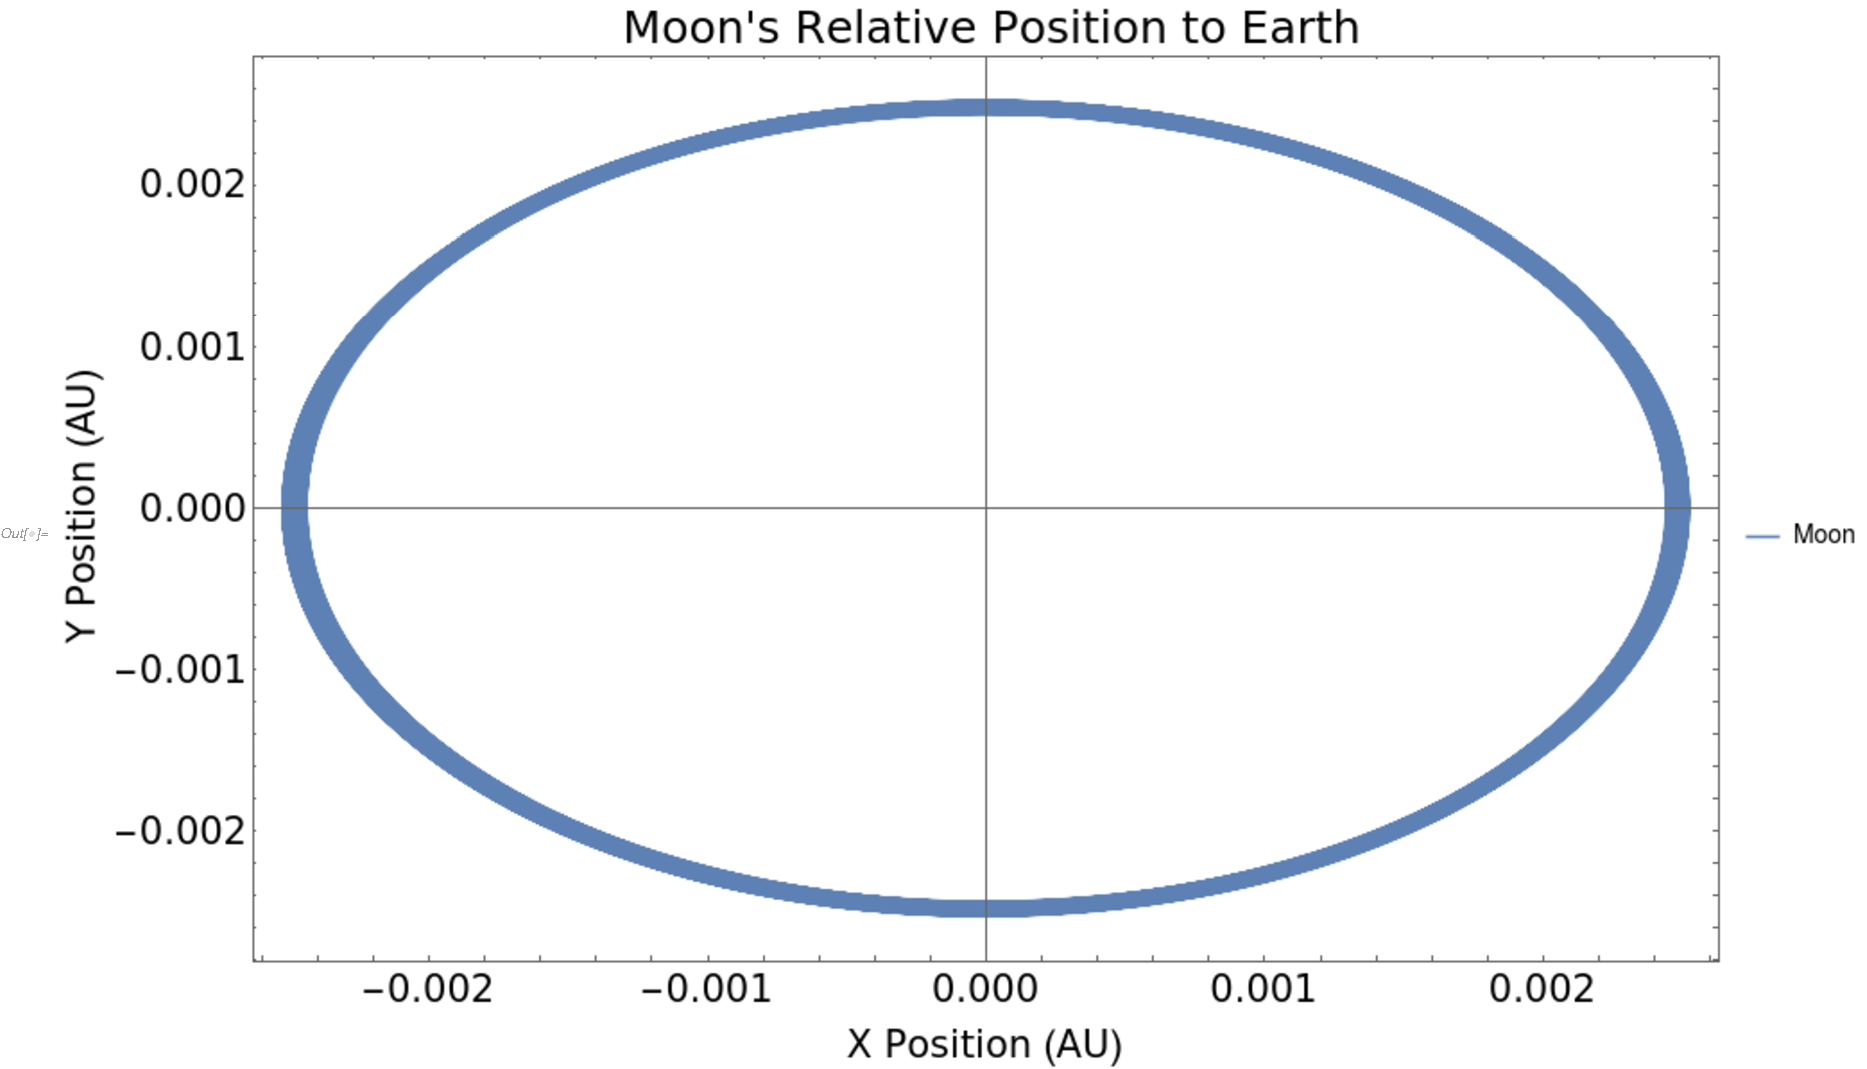
\includegraphics[width=0.5\textwidth]{p1-1b.pdf}
	\end{center}
	\caption{}
\label{fig:qual}
\end{figure}
\FloatBarrier

We can see the ebb and flow of the moons orbit clearly in the Graphic below. There is a gentle trend overall for the moon to drift away from the earth.

\begin{figure}[!htb]
	\begin{center}
		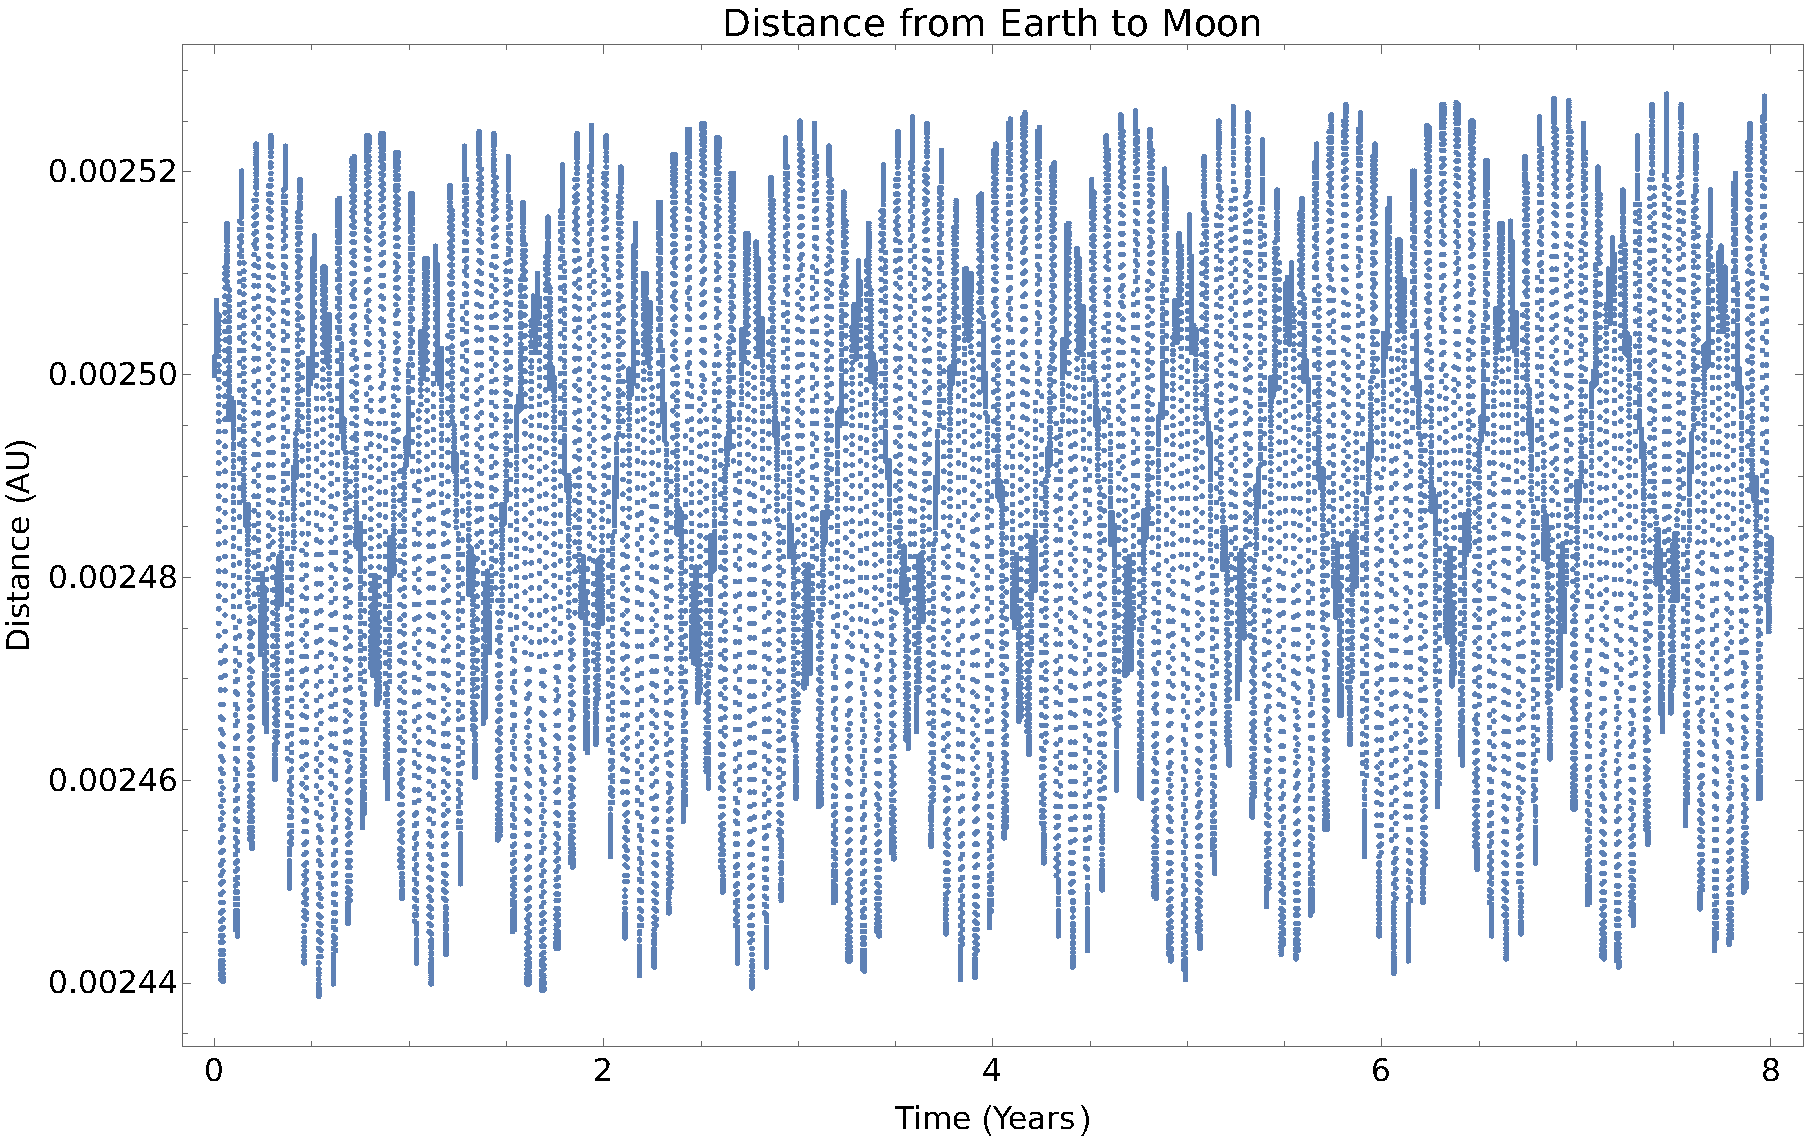
\includegraphics[width=0.5\textwidth]{p1-1c.pdf}
	\end{center}
	\caption{}
\label{fig:qual}
\end{figure}
\FloatBarrier


\begin{figure}[!htb]
	\begin{center}
		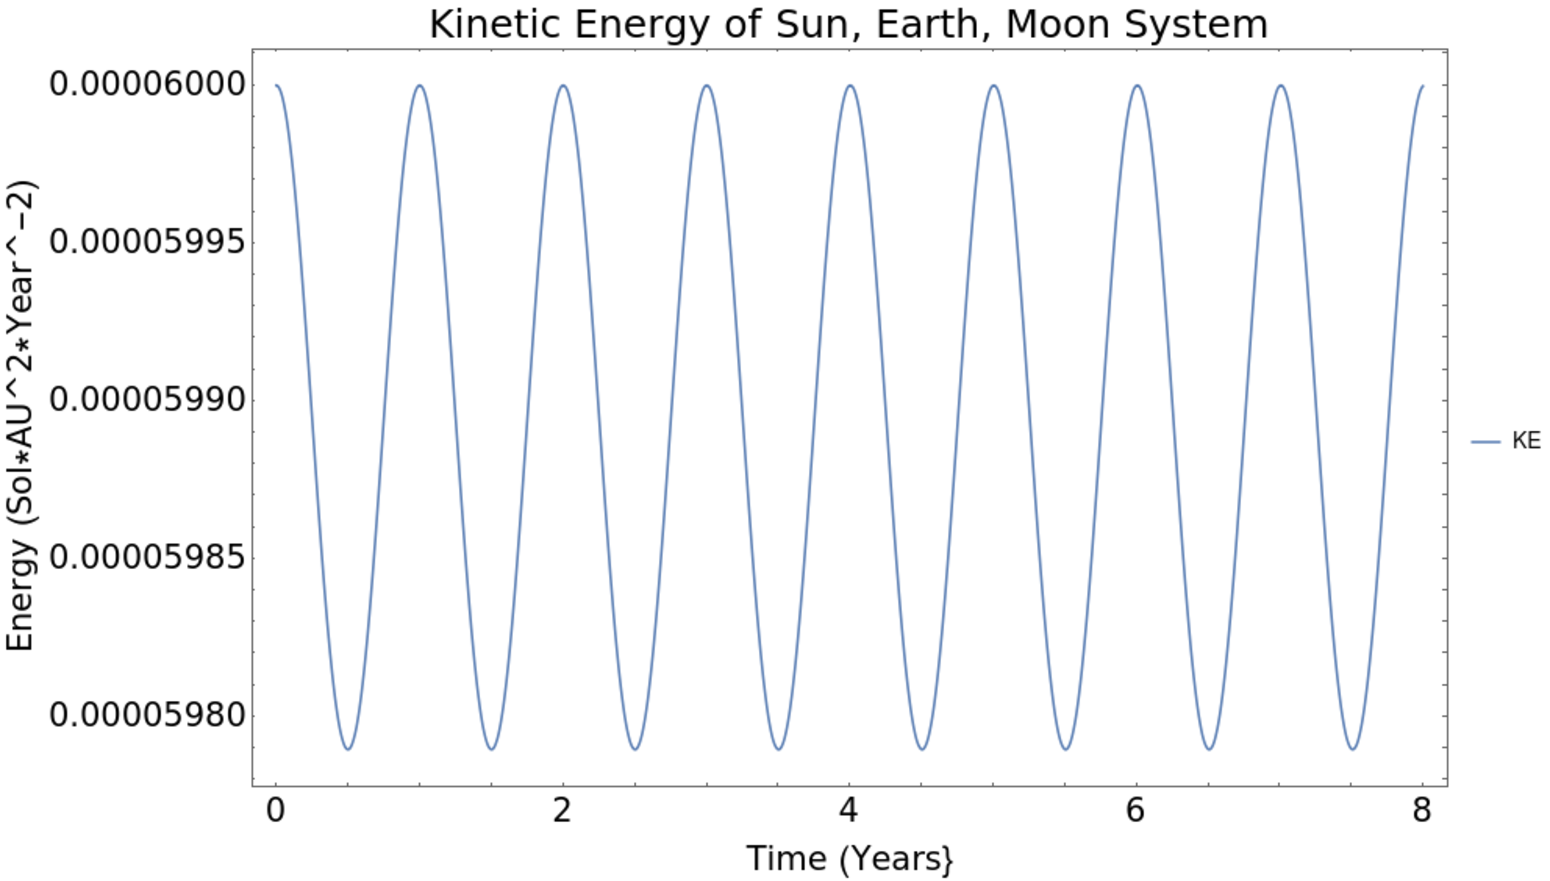
\includegraphics[width=0.5\textwidth]{p1-1d.pdf}
	\end{center}
	\caption{}
\label{fig:qual}
\end{figure}
\FloatBarrier


\begin{figure}[!htb]
	\begin{center}
		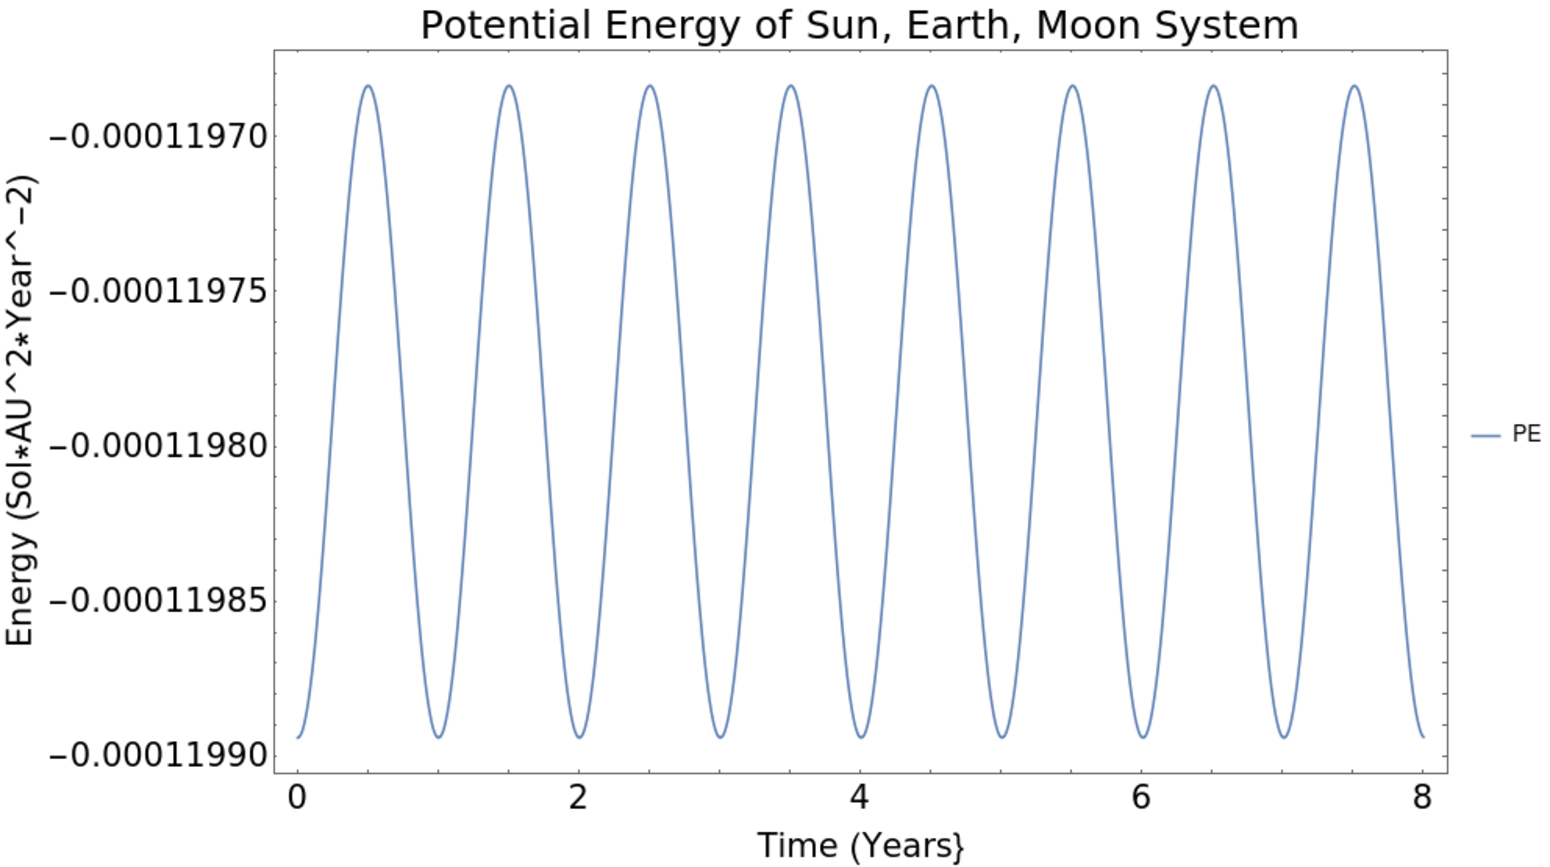
\includegraphics[width=0.5\textwidth]{p1-1e.pdf}
	\end{center}
	\caption{}
\label{fig:qual}
\end{figure}
\FloatBarrier


\begin{figure}[!htb]
	\begin{center}
		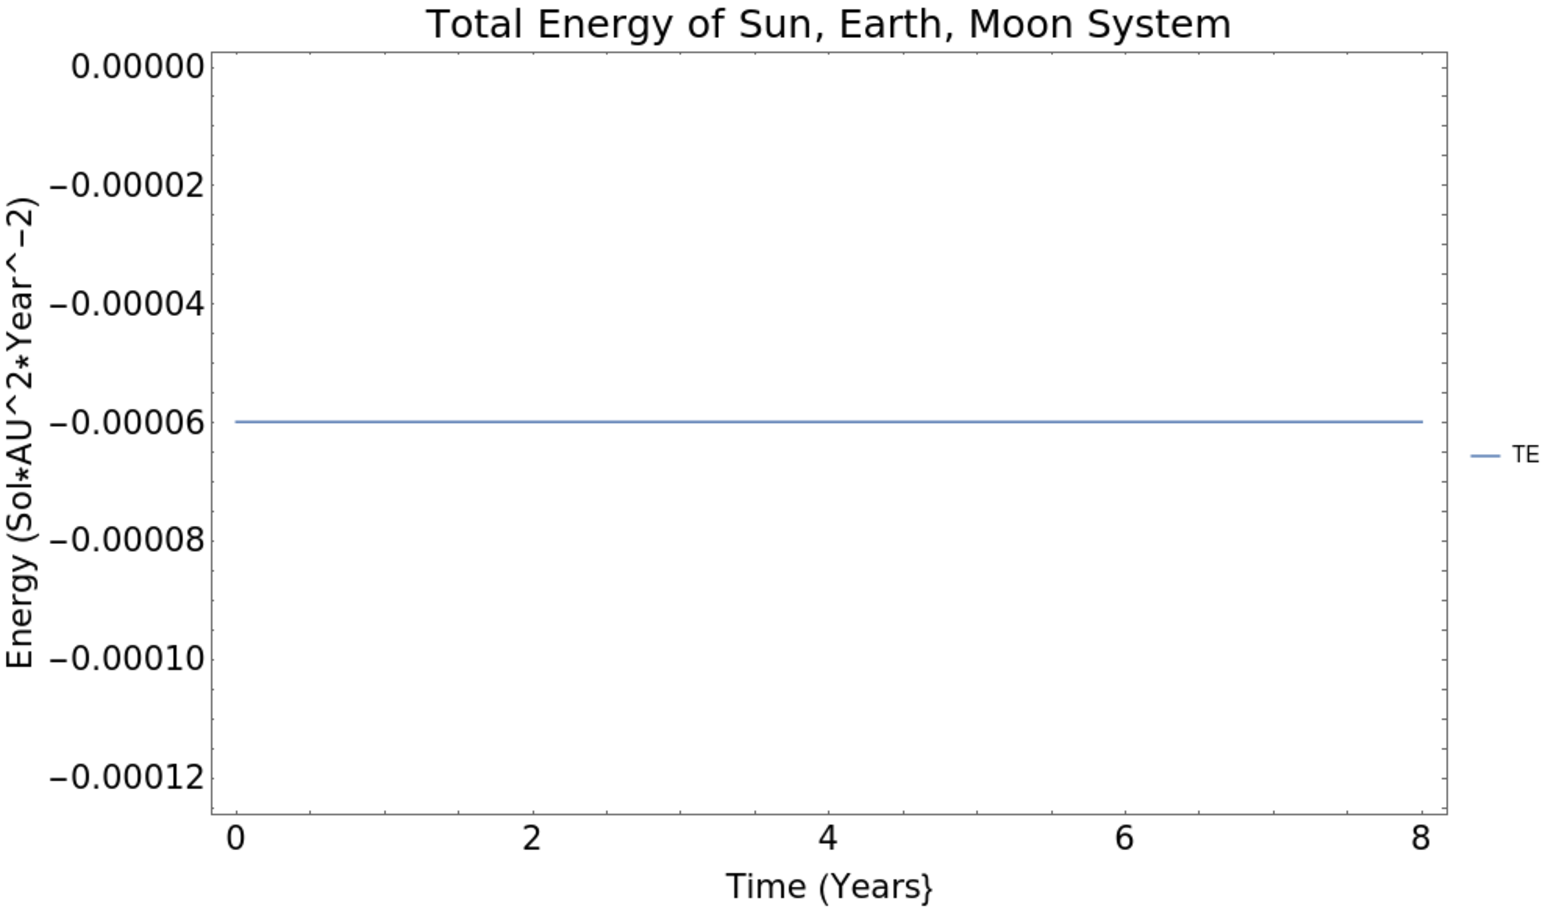
\includegraphics[width=0.5\textwidth]{p1-1f.pdf}
	\end{center}
	\caption{}
\label{fig:qual}
\end{figure}
\FloatBarrier

\begin{figure}[!htb]
	\begin{center}
		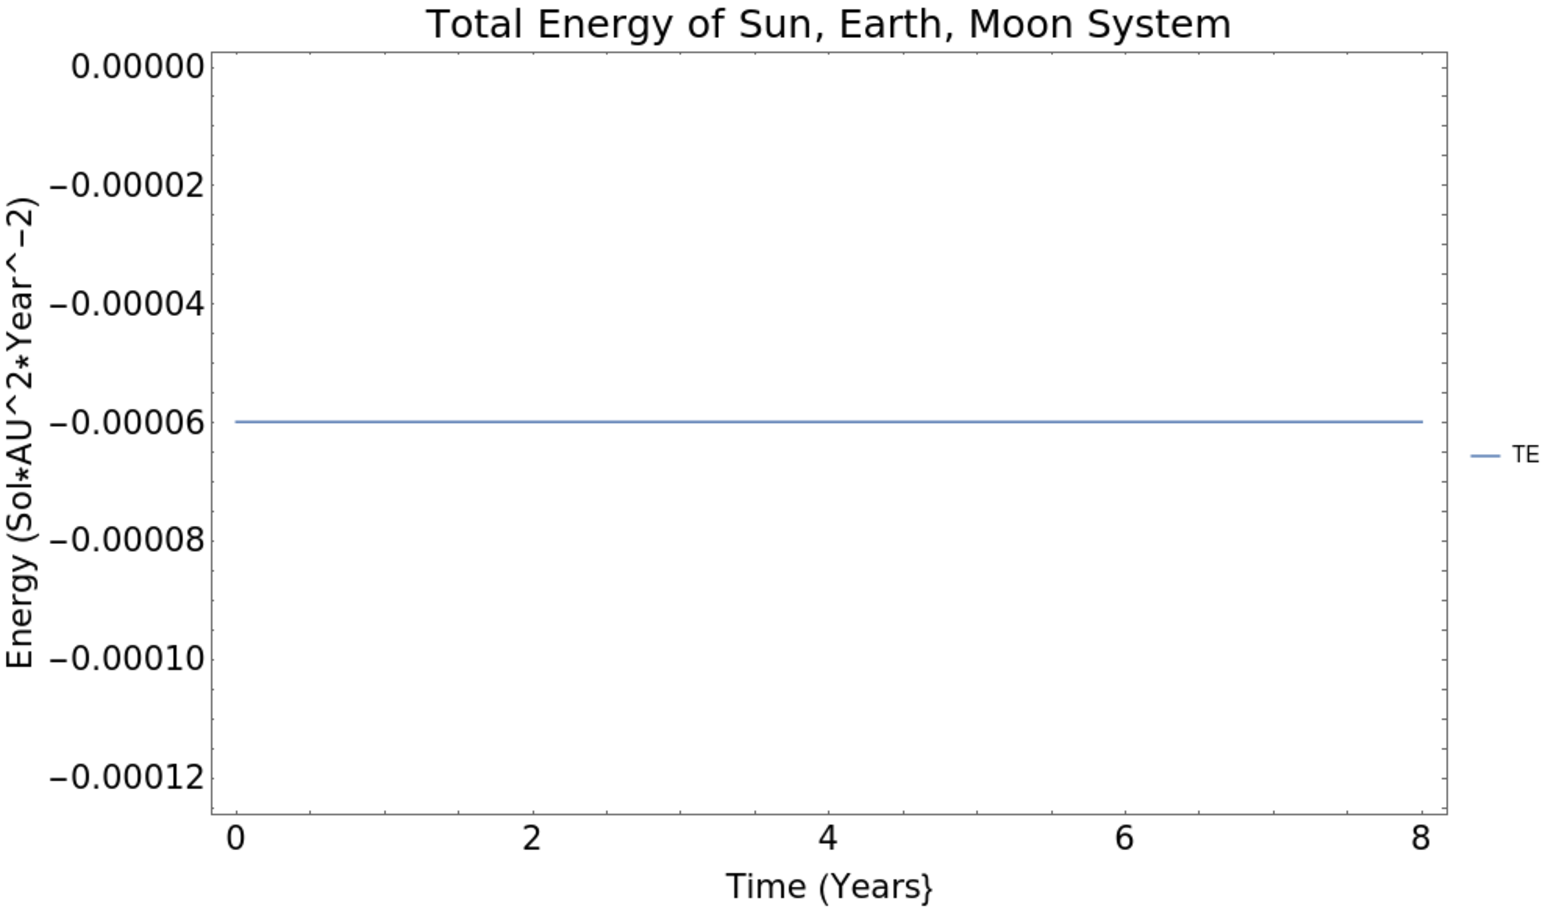
\includegraphics[width=0.5\textwidth]{p1-1f.pdf}
	\end{center}
	\caption{}
\label{fig:qual}
\end{figure}
\FloatBarrier

\subsubsection{2}

What Happens if we change the parameters of the Earth Sun and Moon?
Below are similar plots, but instead of the actual values of the Sun, Earth and Moon, I plotted $M_1 = 1, M_2 = 10^{-2}, M_3 = 10^{-4}, r_{23} = 0,06$ AU. 

\begin{figure}[!htb]
	\begin{center}
		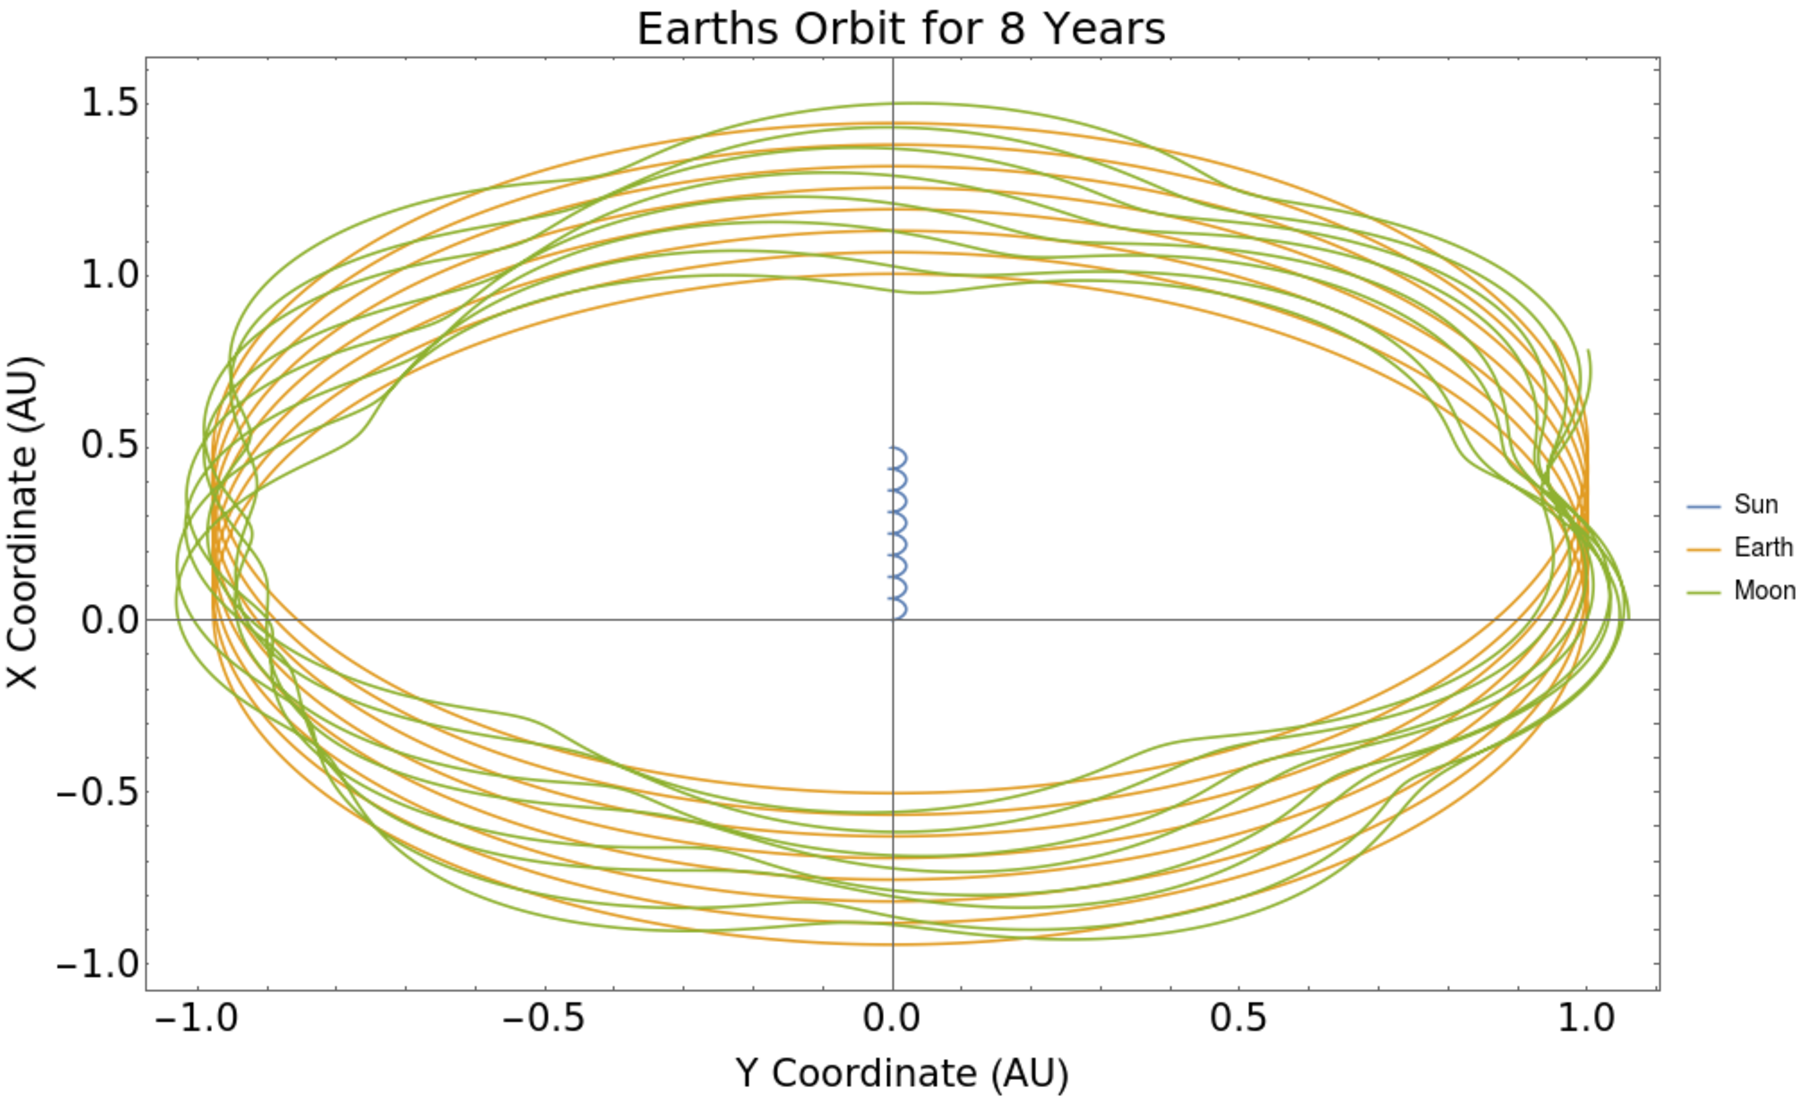
\includegraphics[width=0.5\textwidth]{p1-2a.pdf}
	\end{center}
	\caption{}
\label{fig:qual}
\end{figure}
\FloatBarrier

Over 8 Years the Moon slowly drifts towards, and away from the earth with a net movement away.

\begin{figure}[!htb]
	\begin{center}
		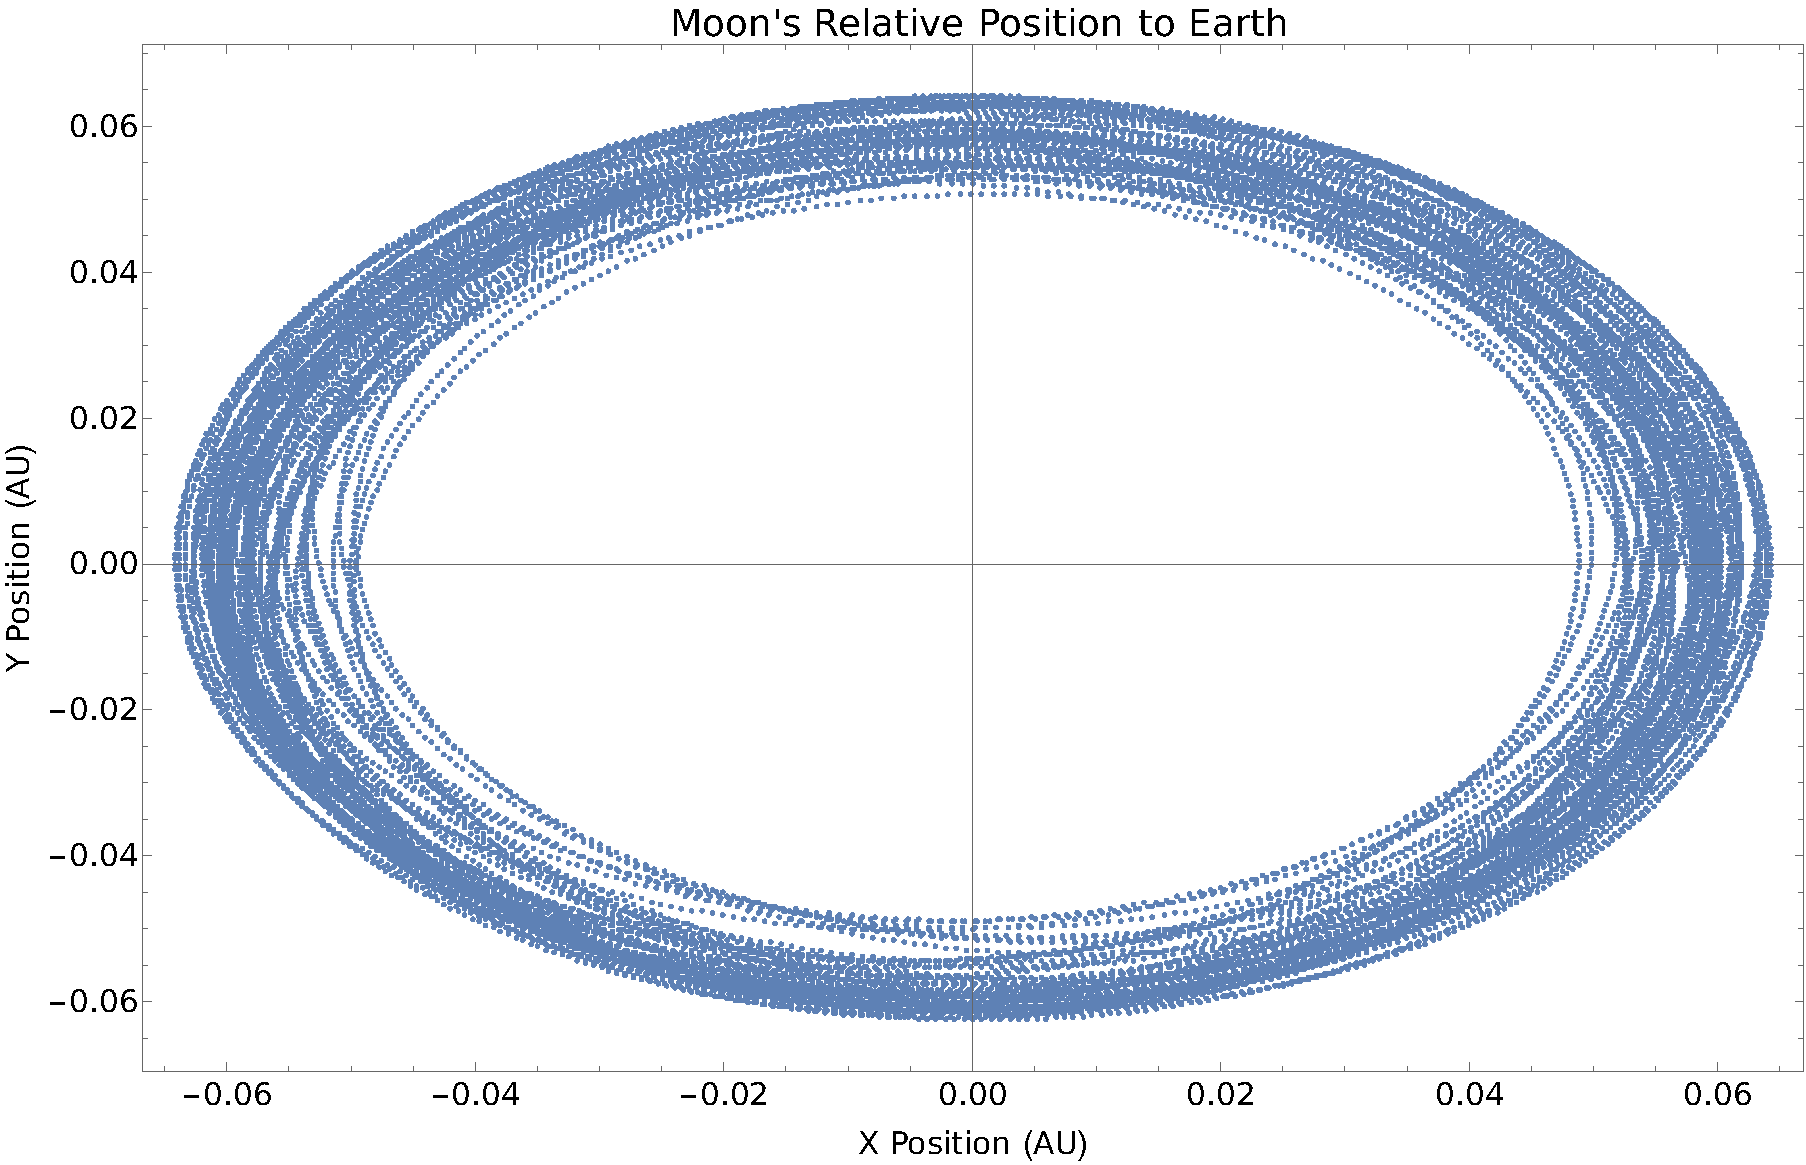
\includegraphics[width=0.5\textwidth]{p1-2b.pdf}
	\end{center}
	\caption{}
\label{fig:qual}
\end{figure}
\FloatBarrier

We can see the ebb and flow of the moons orbit clearly in the Graphic below. There is a gentle trend overall for the moon to drift away from the earth.

\begin{figure}[!htb]
	\begin{center}
		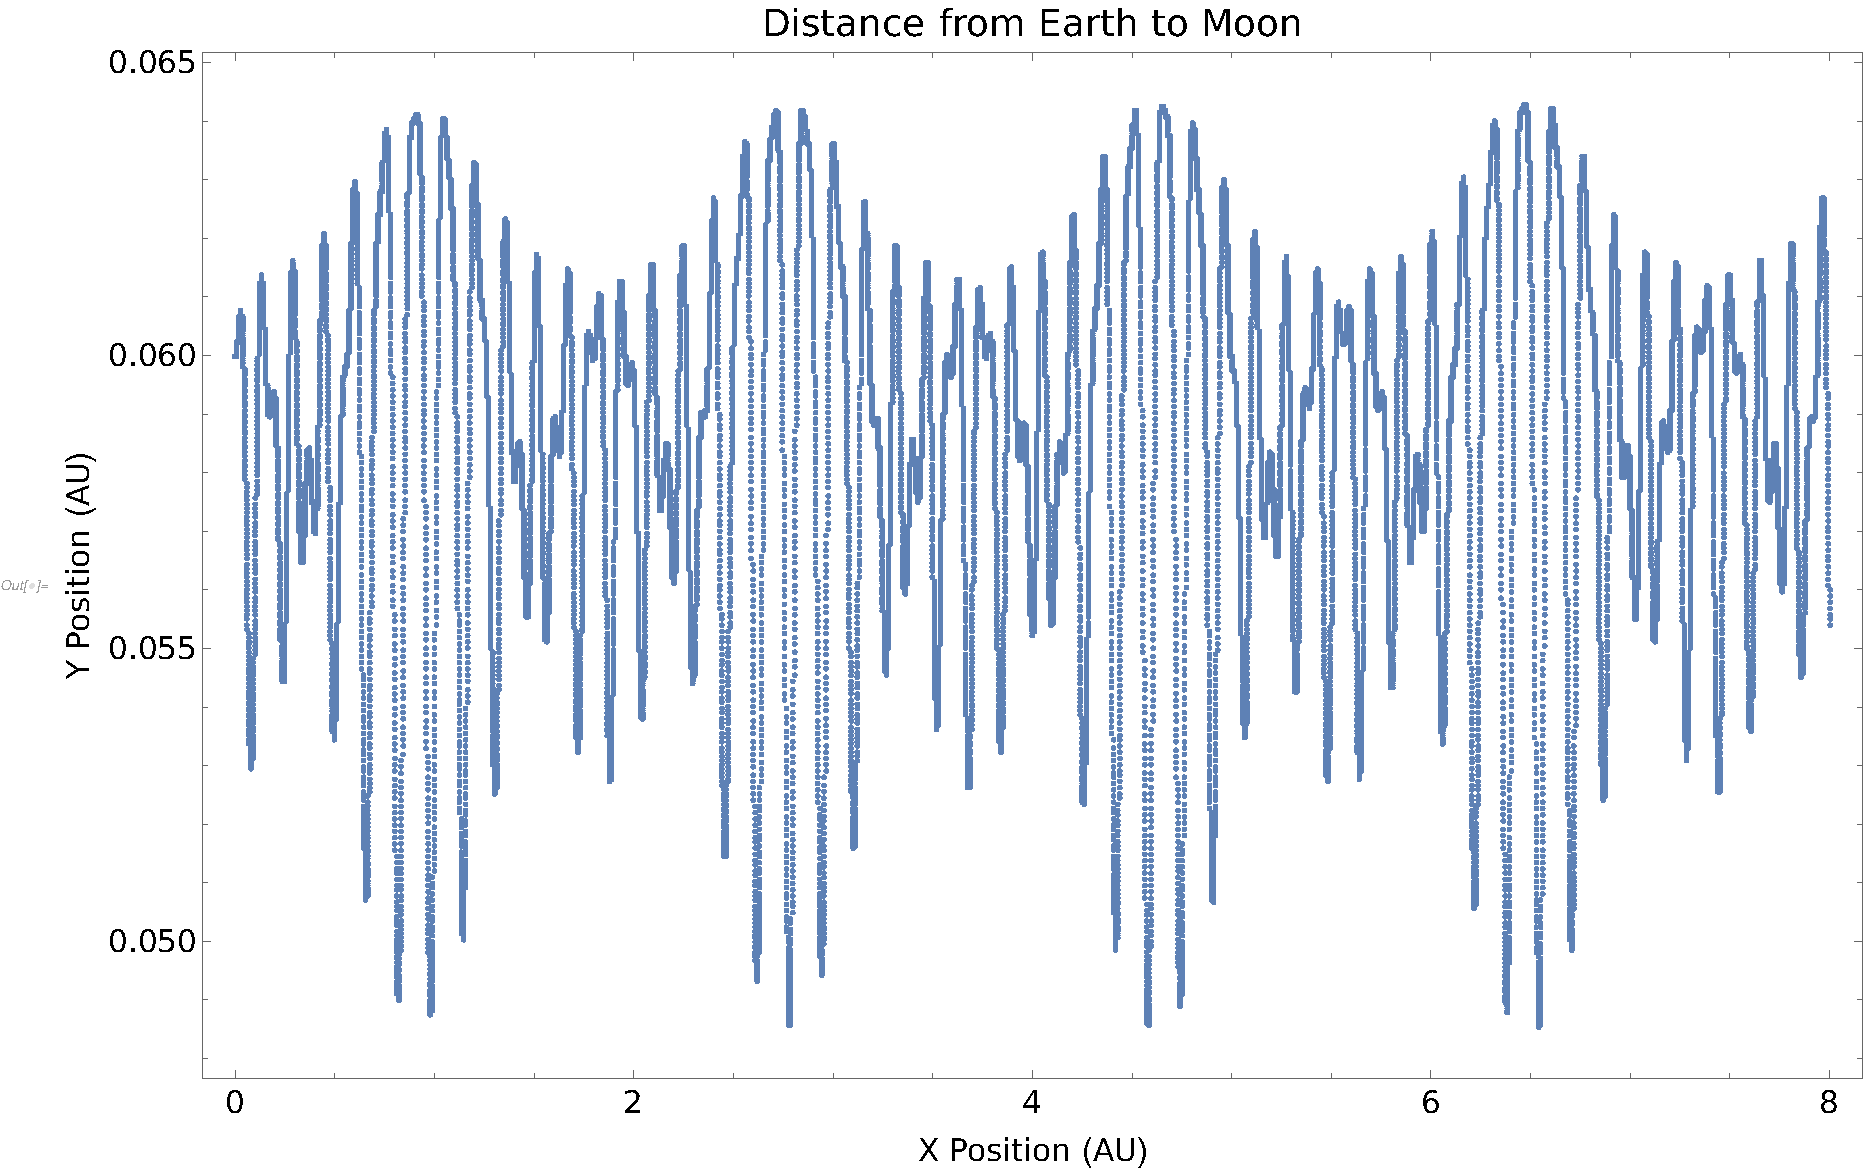
\includegraphics[width=0.5\textwidth]{p1-2c.pdf}
	\end{center}
	\caption{}
\label{fig:qual}
\end{figure}
\FloatBarrier


\begin{figure}[!htb]
	\begin{center}
		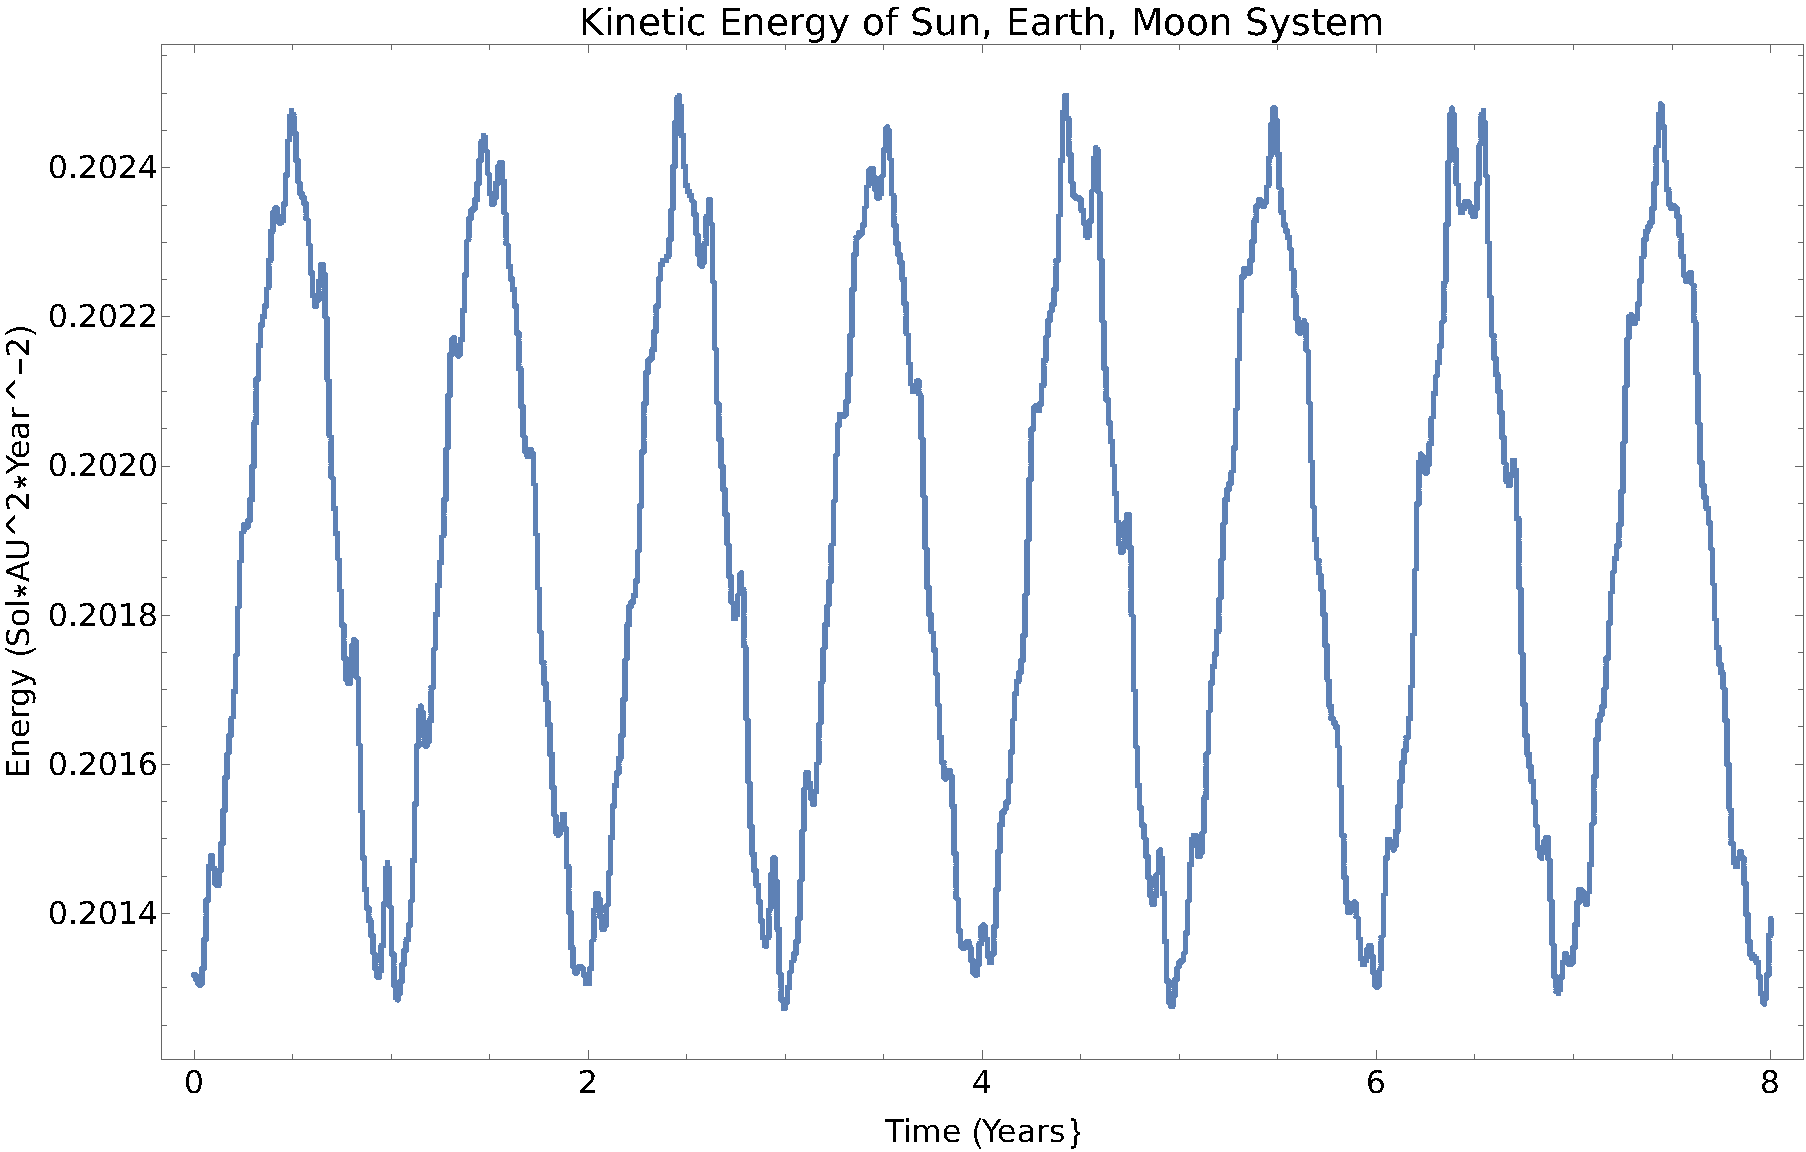
\includegraphics[width=0.5\textwidth]{p1-2d.pdf}
	\end{center}
	\caption{}
\label{fig:qual}
\end{figure}
\FloatBarrier


\begin{figure}[!htb]
	\begin{center}
		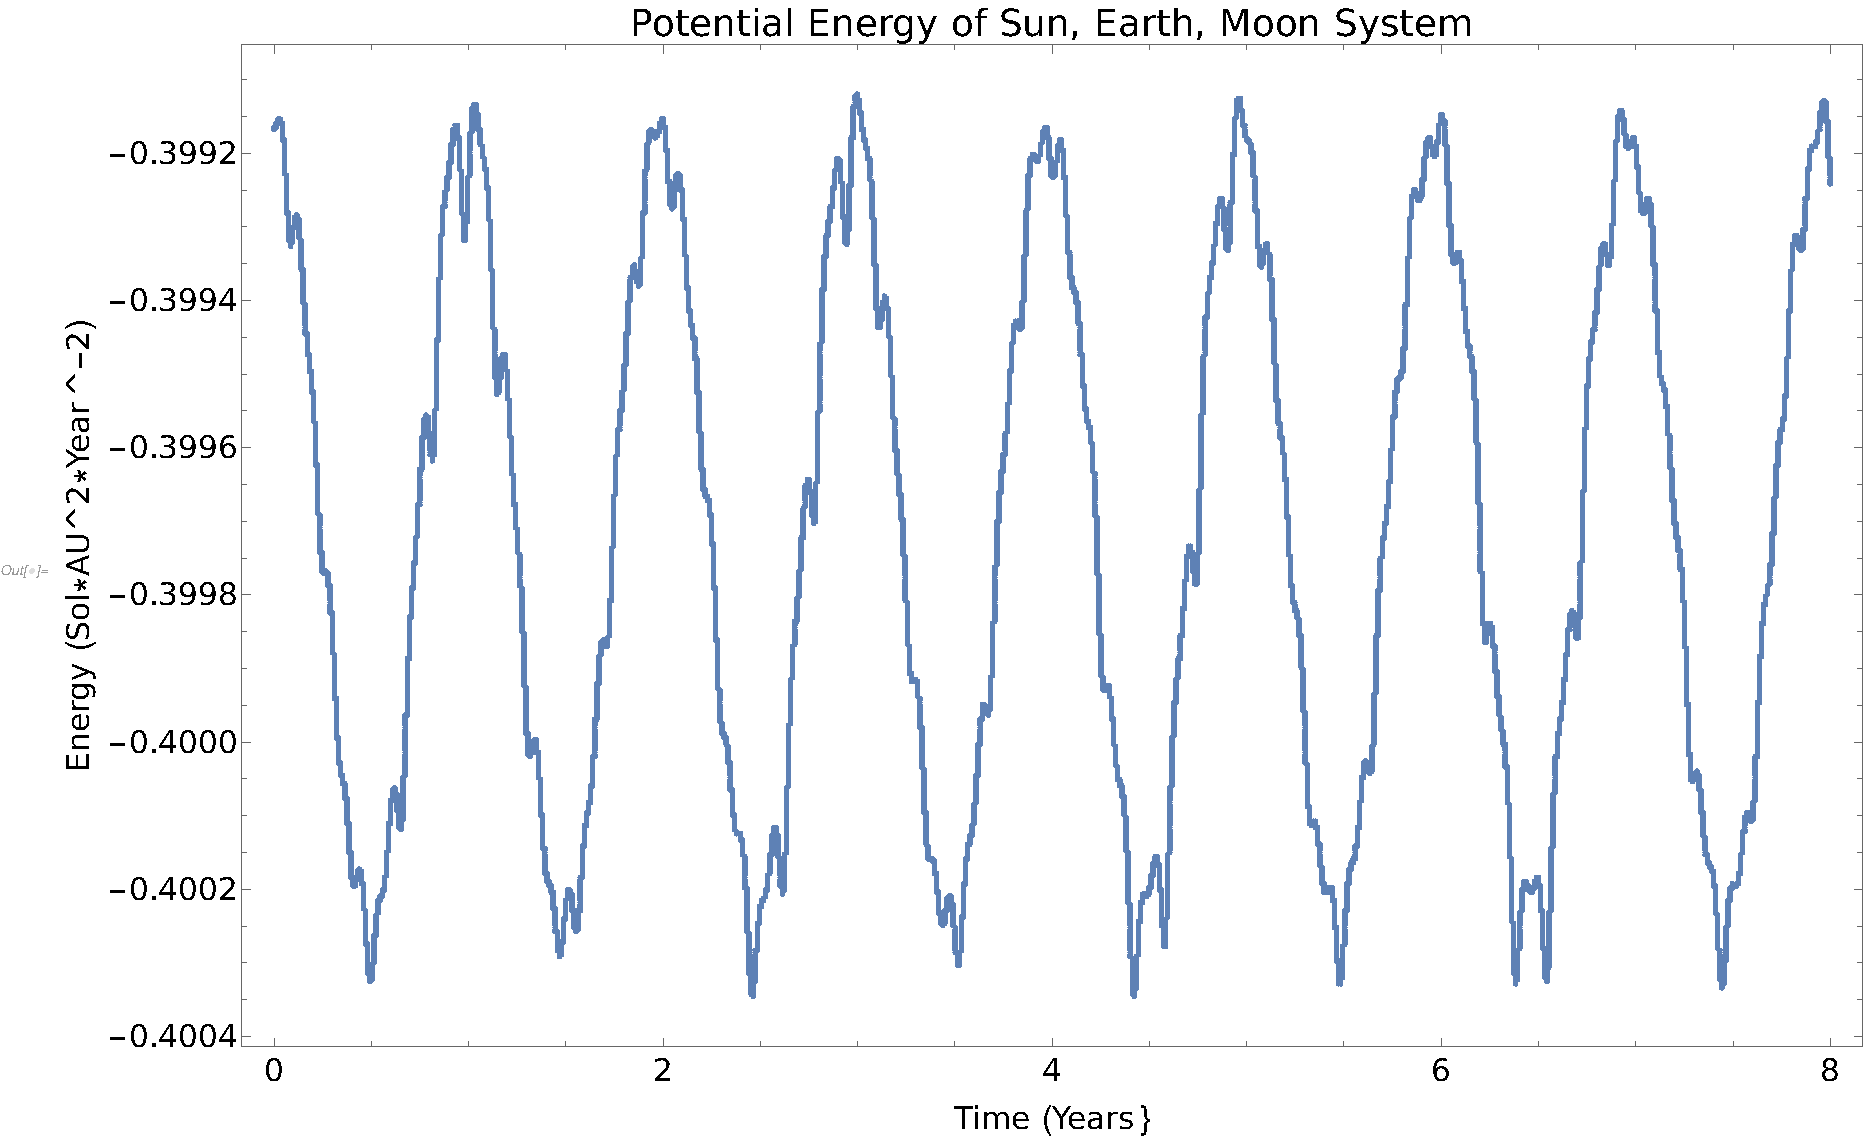
\includegraphics[width=0.5\textwidth]{p1-2e.pdf}
	\end{center}
	\caption{}
\label{fig:qual}
\end{figure}
\FloatBarrier


\begin{figure}[!htb]
	\begin{center}
		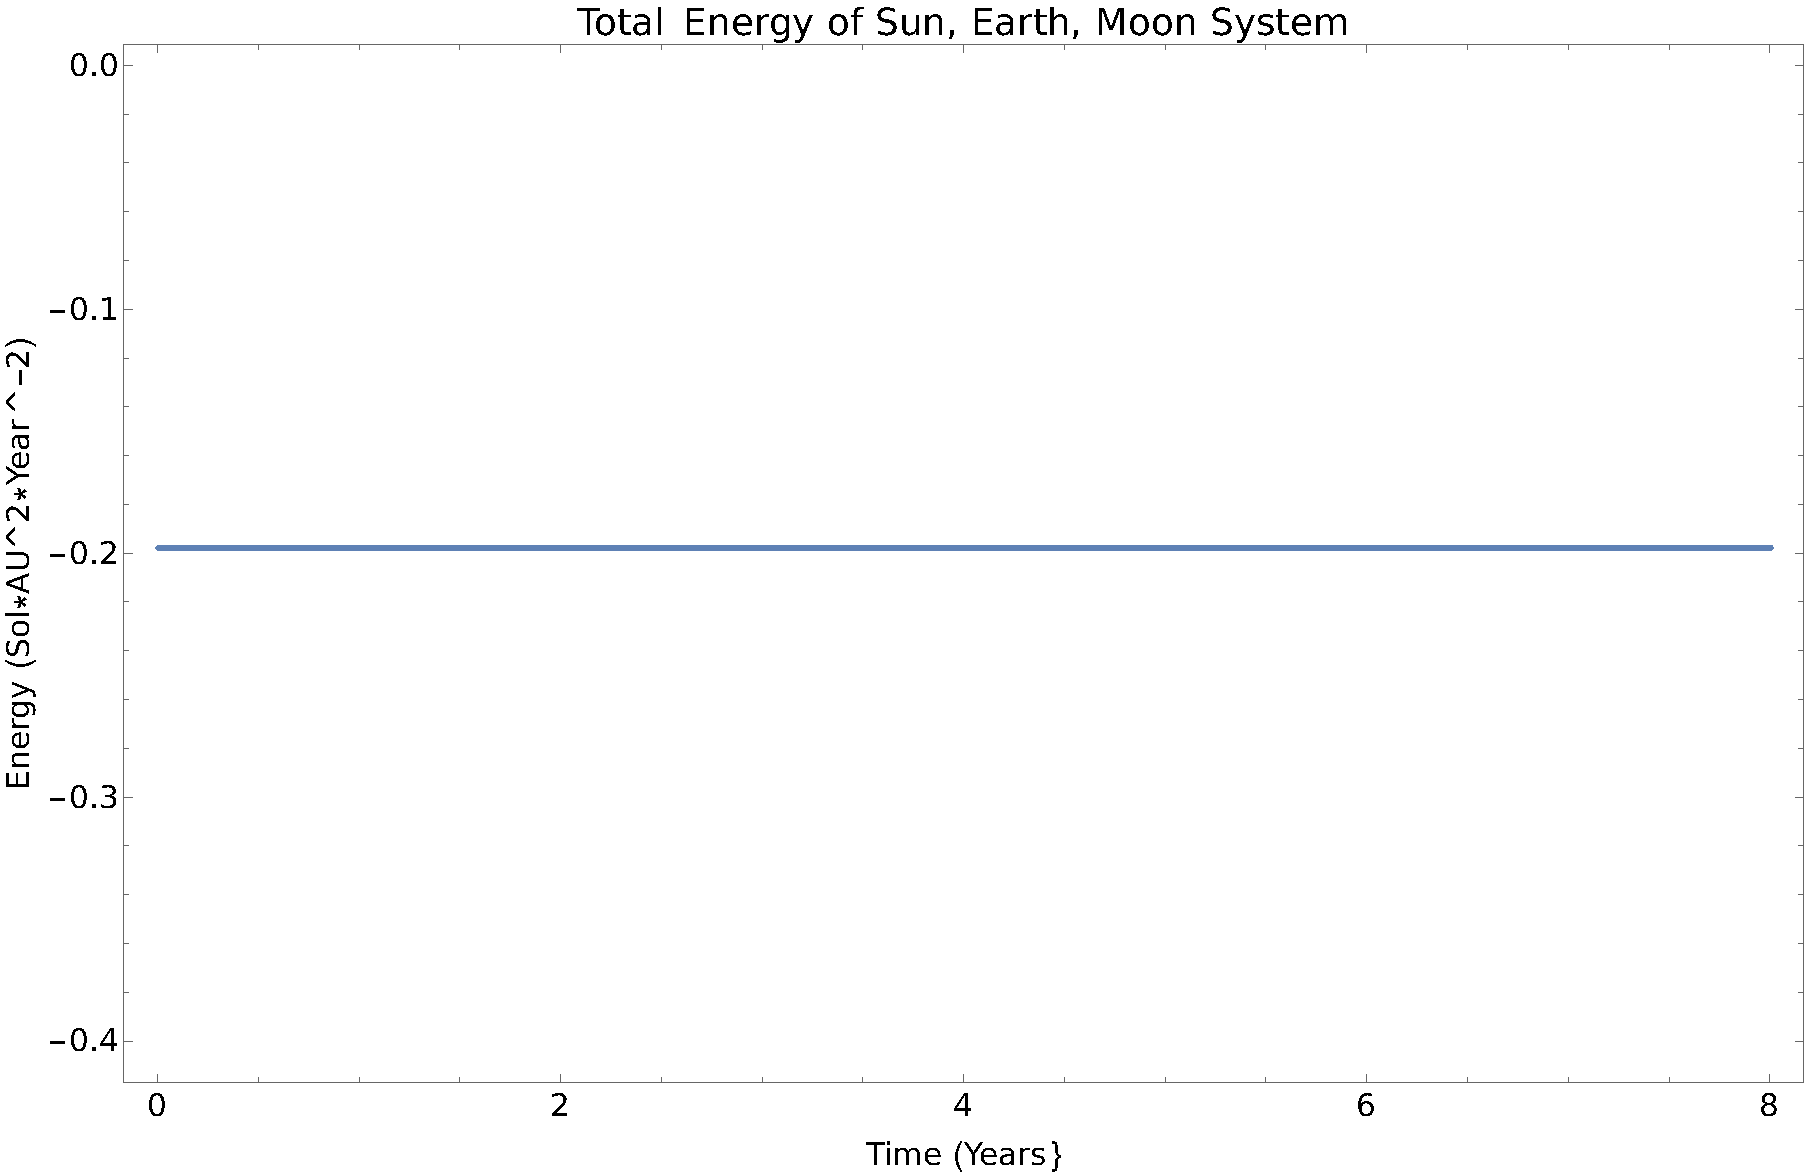
\includegraphics[width=0.5\textwidth]{p1-2f.pdf}
	\end{center}
	\caption{}
\label{fig:qual}
\end{figure}
\FloatBarrier

\subsubsection{3}

Plotted for $M_1 = 1, M_2 = 10^{-2}, M_3 = 10^{-4}, r_{23} = 0,08$ AU. 

\begin{figure}[!htb]
	\begin{center}
		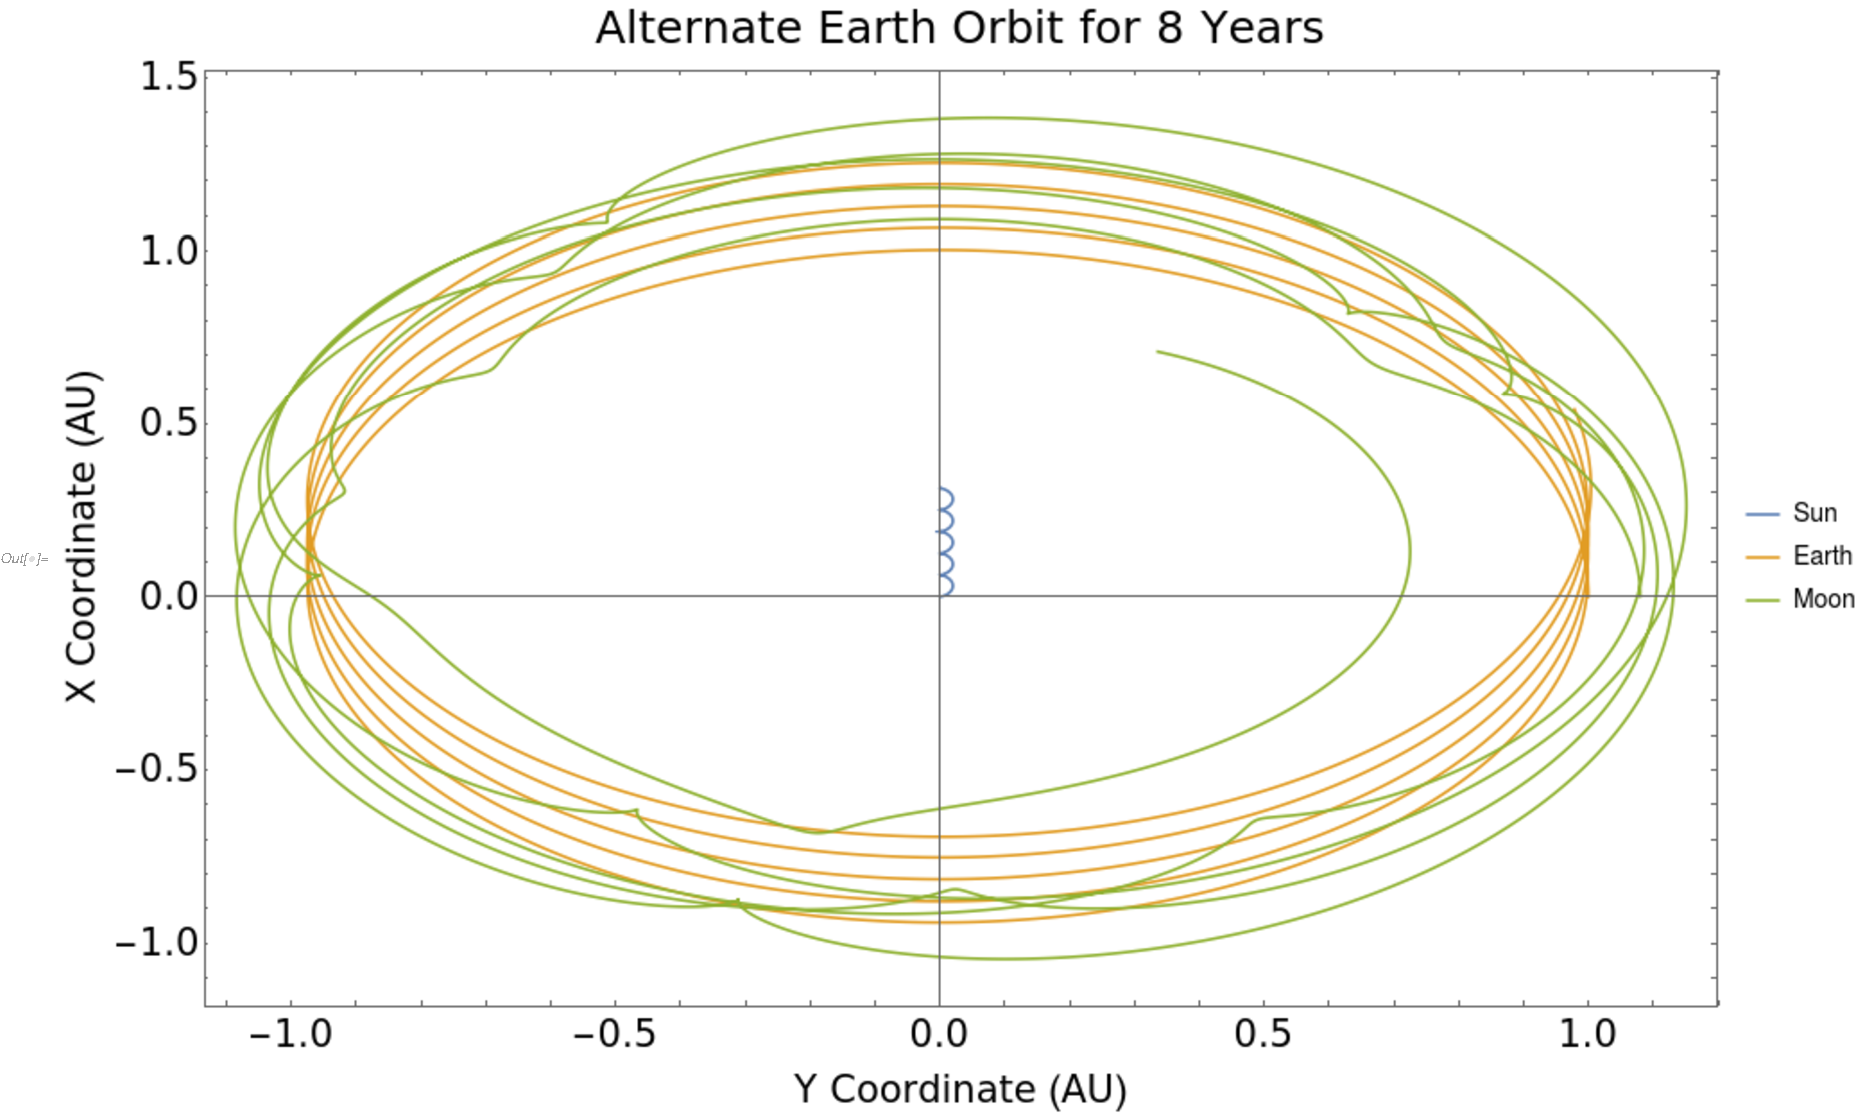
\includegraphics[width=0.5\textwidth]{p1-3a.pdf}
	\end{center}
	\caption{}
\label{fig:qual}
\end{figure}
\FloatBarrier

Over 8 Years the Moon slowly drifts towards, and away from the earth with a net movement away.

\begin{figure}[!htb]
	\begin{center}
		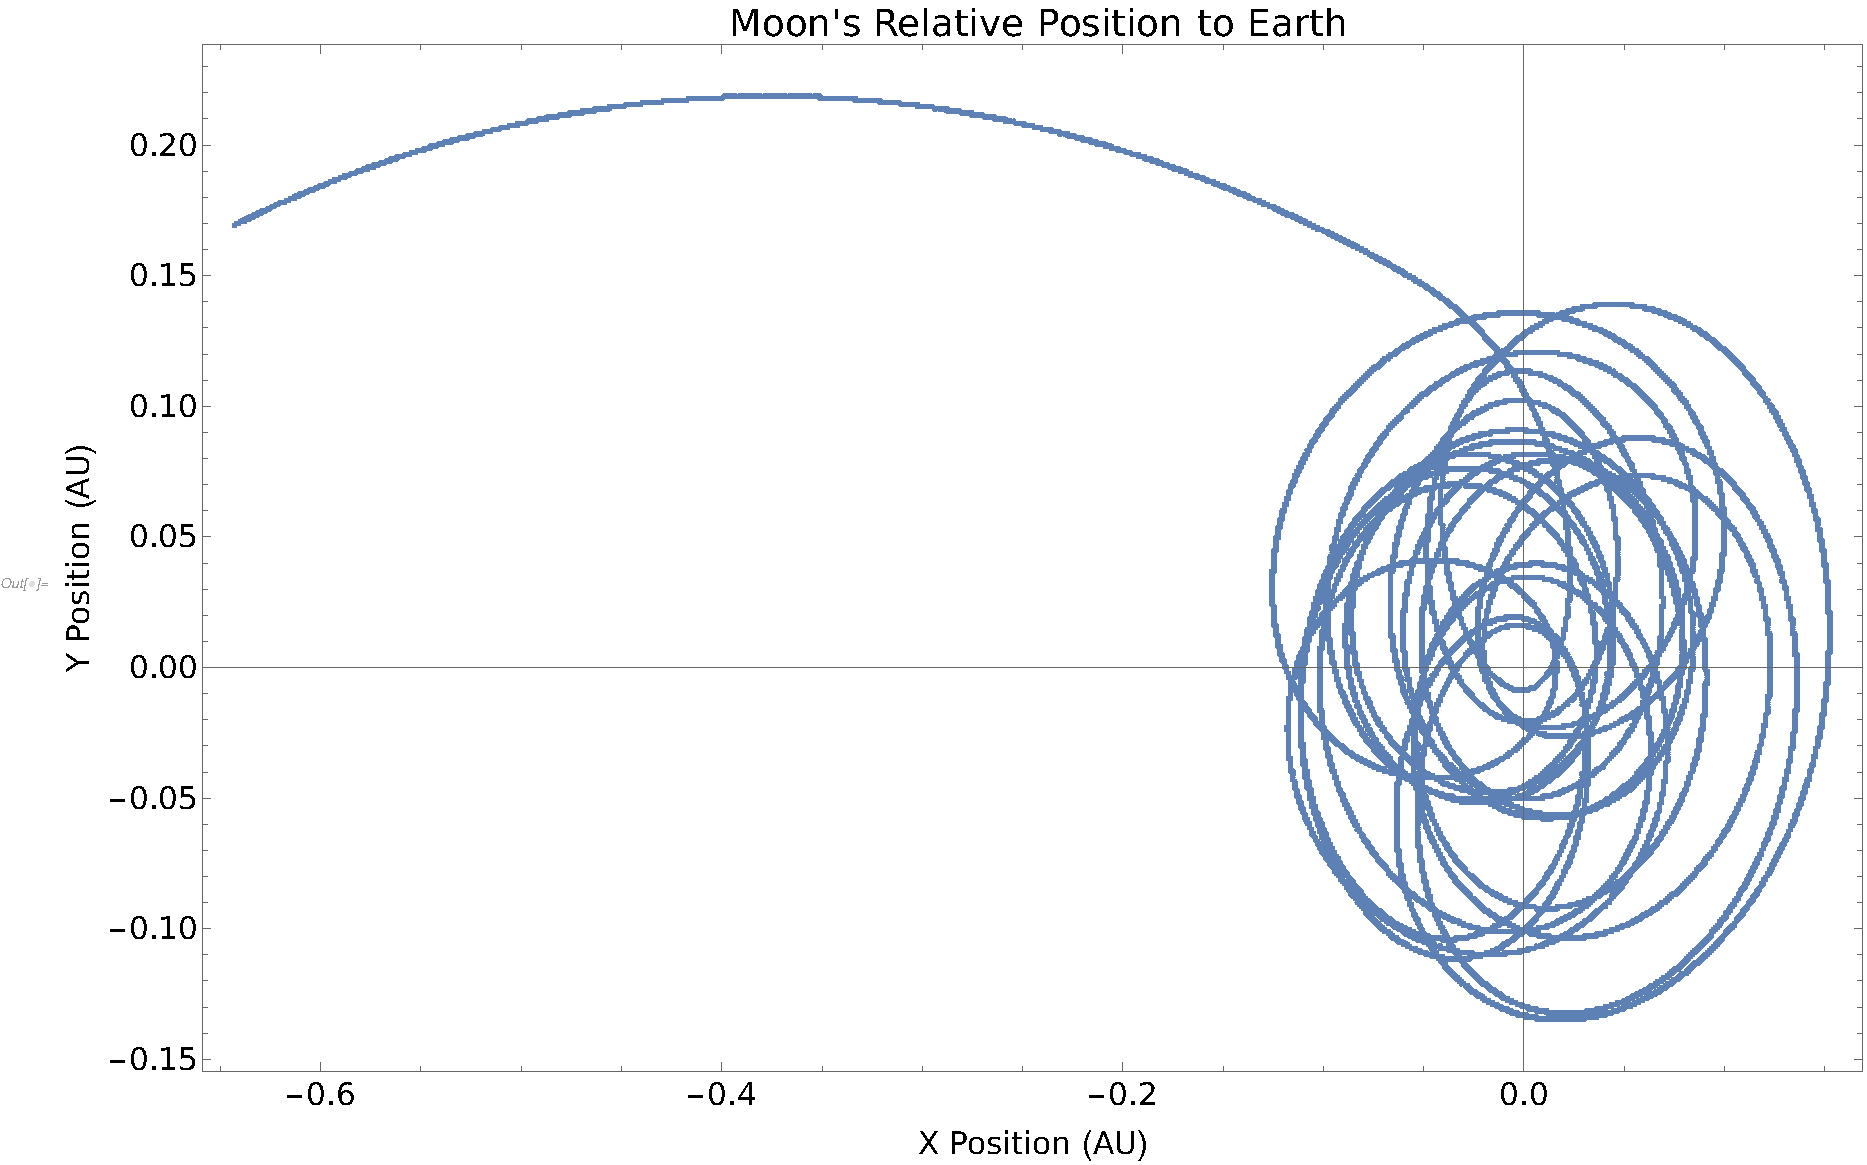
\includegraphics[width=0.5\textwidth]{p1-3b.pdf}
	\end{center}
	\caption{}
\label{fig:qual}
\end{figure}
\FloatBarrier

We can see the ebb and flow of the moons orbit clearly in the Graphic below. There is a gentle trend overall for the moon to drift away from the earth.

\begin{figure}[!htb]
	\begin{center}
		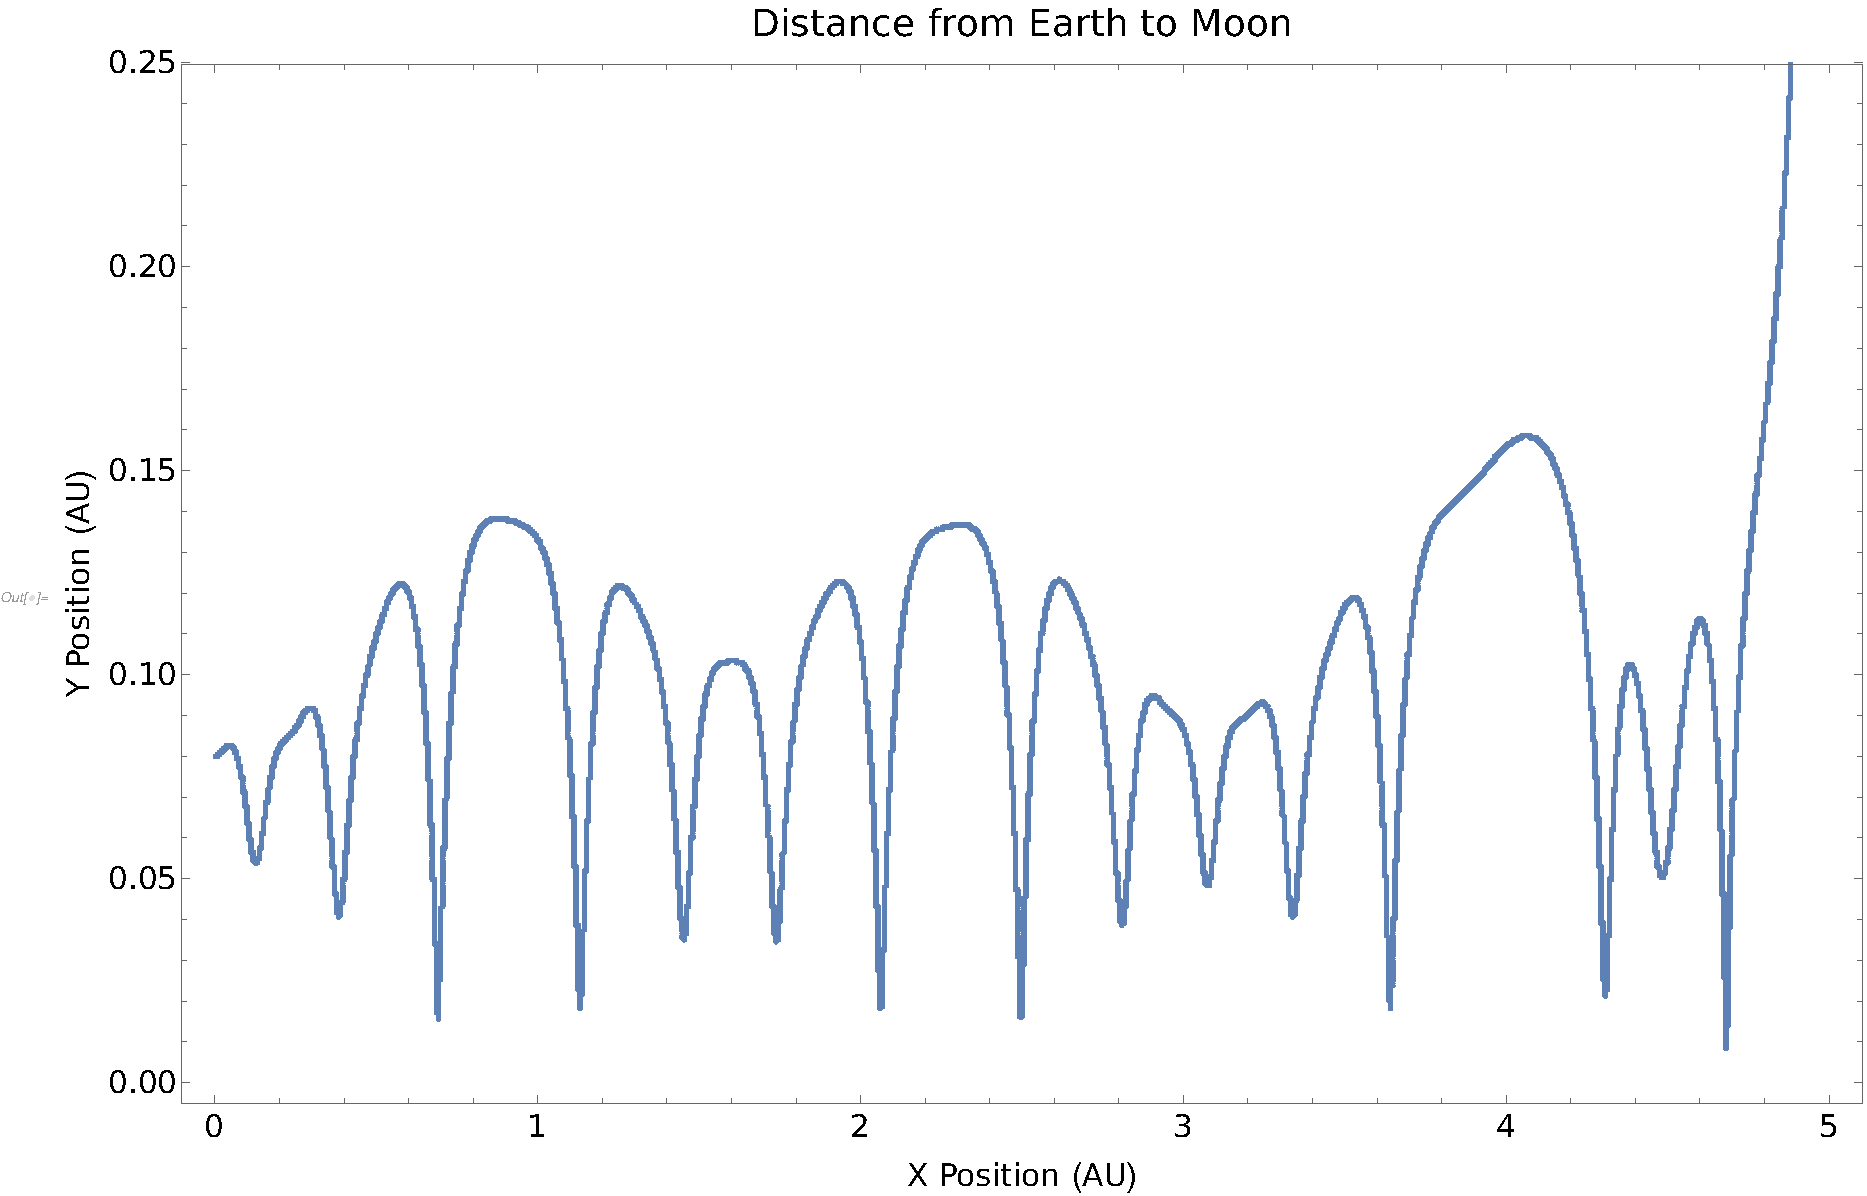
\includegraphics[width=0.5\textwidth]{p1-3c.pdf}
	\end{center}
	\caption{}
\label{fig:qual}
\end{figure}
\FloatBarrier


\begin{figure}[!htb]
	\begin{center}
		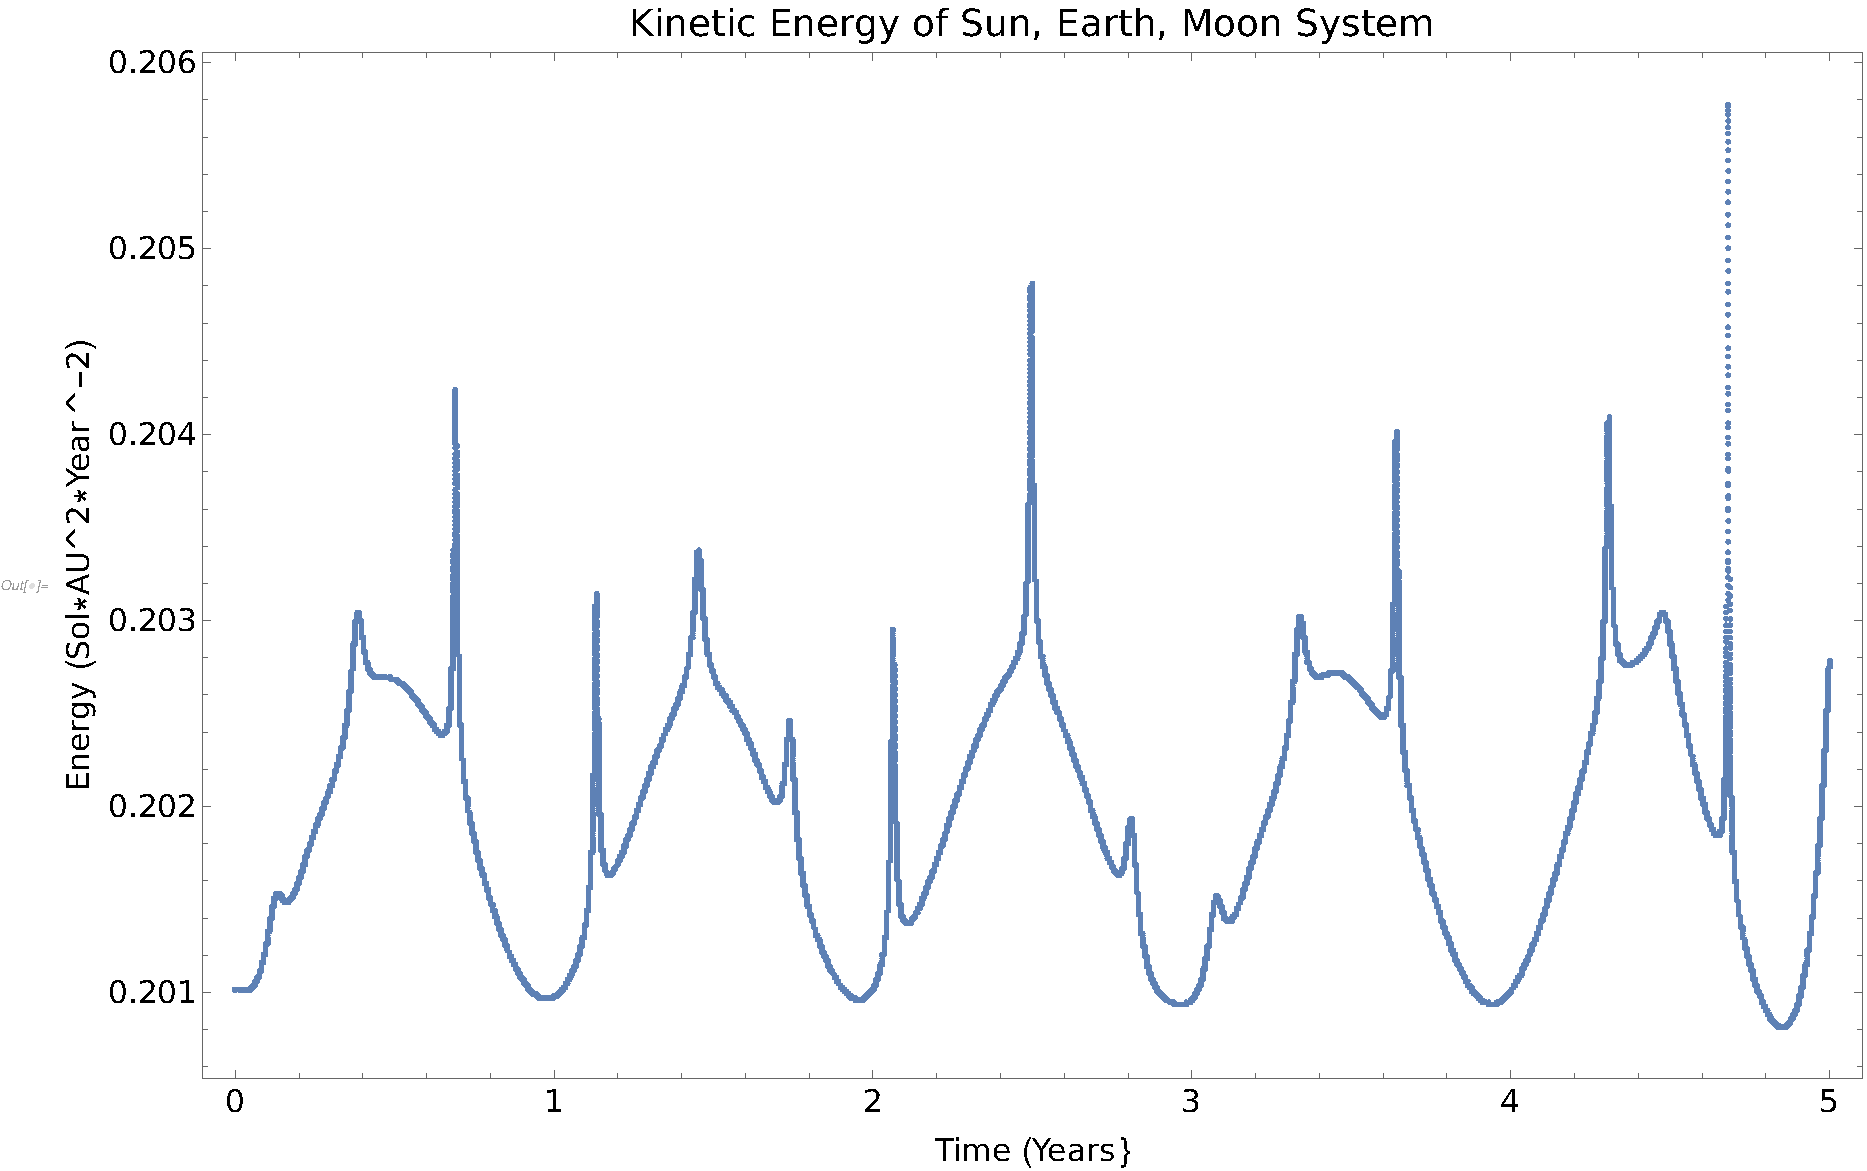
\includegraphics[width=0.5\textwidth]{p1-3d.pdf}
	\end{center}
	\caption{}
\label{fig:qual}
\end{figure}
\FloatBarrier


\begin{figure}[!htb]
	\begin{center}
		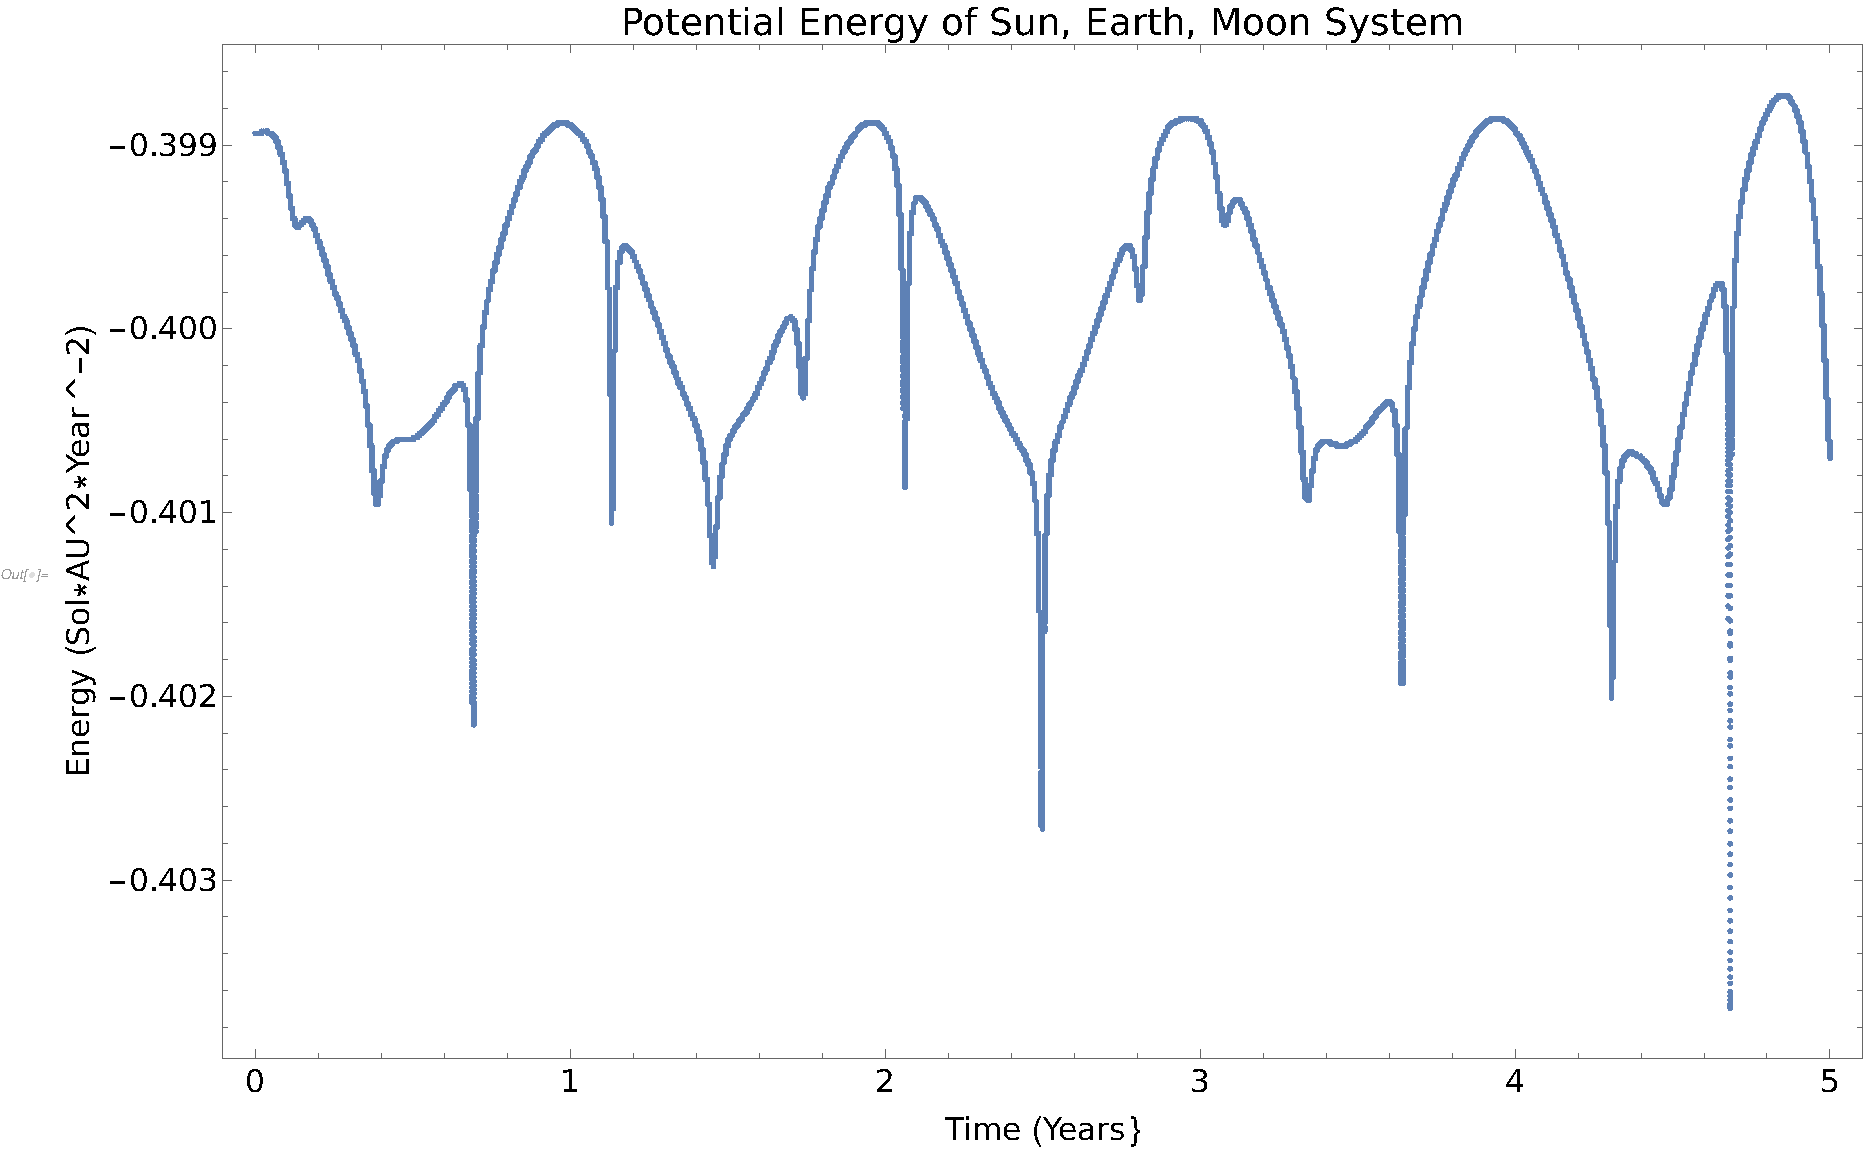
\includegraphics[width=0.5\textwidth]{p1-3e.pdf}
	\end{center}
	\caption{}
\label{fig:qual}
\end{figure}
\FloatBarrier


\begin{figure}[!htb]
	\begin{center}
		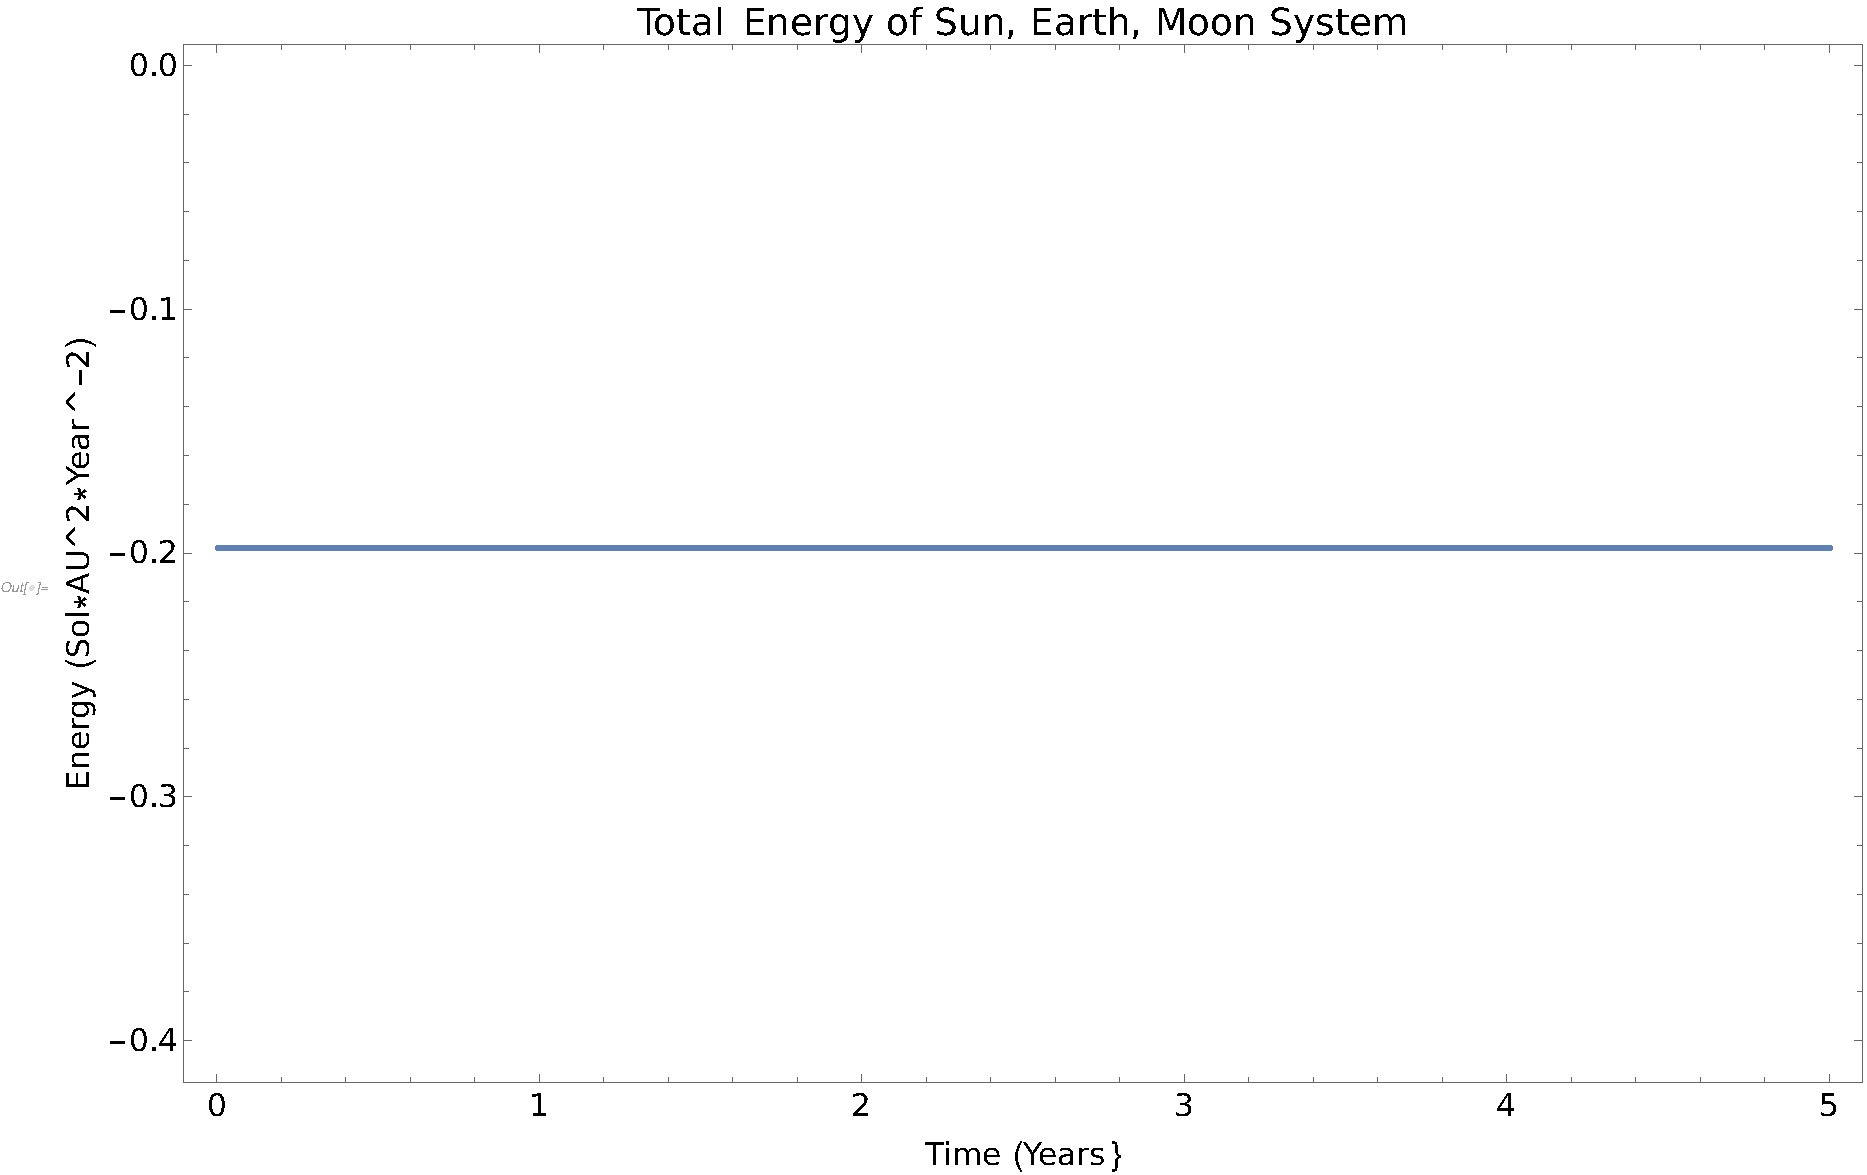
\includegraphics[width=0.5\textwidth]{p1-3f.pdf}
	\end{center}
	\caption{}
\label{fig:qual}
\end{figure}
\FloatBarrier  

\subsubsection{4}

Plotted for $M_1 = 1, M_2 = 10^{-1}, M_3 = 10^{-4}, r_{23} = 0.2$ AU. 

\begin{figure}[!htb]
	\begin{center}
		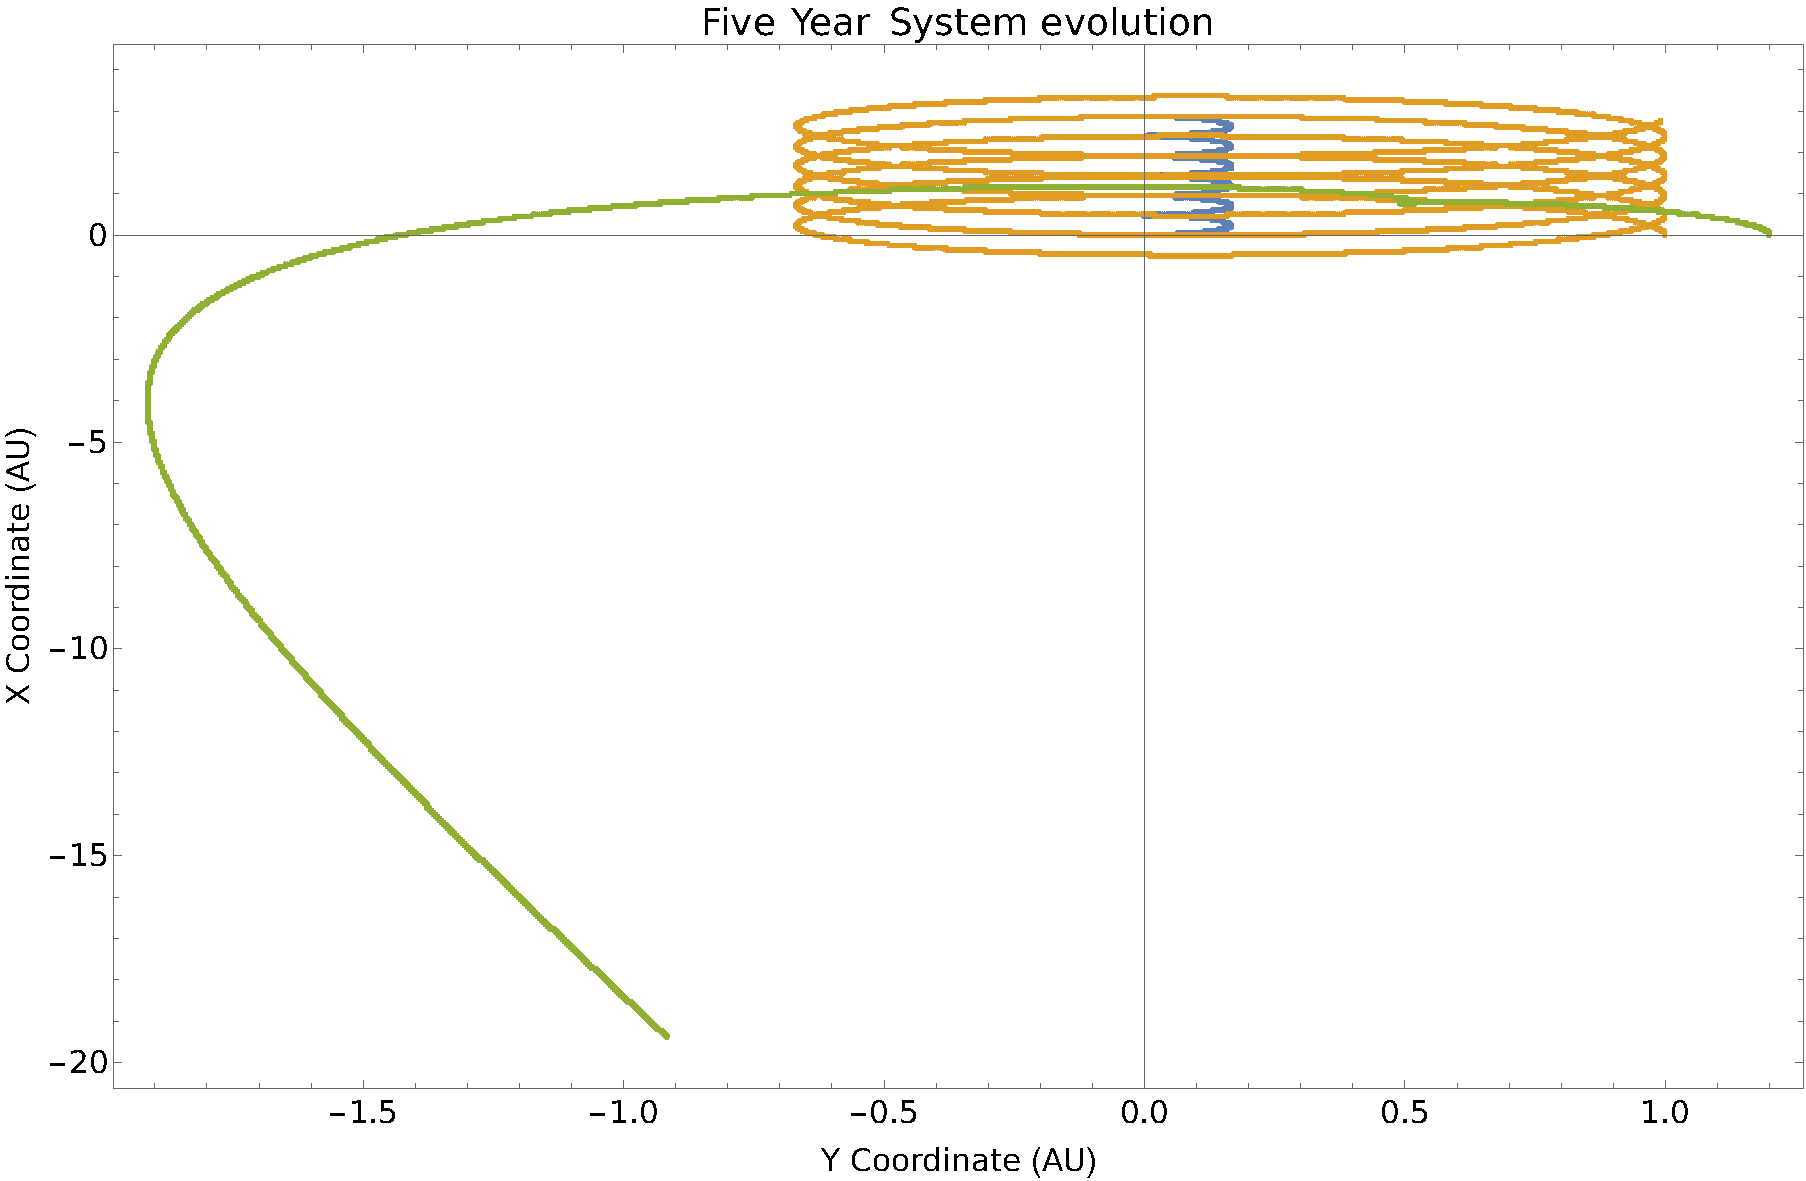
\includegraphics[width=0.5\textwidth]{p1-4a.pdf}
	\end{center}
	\caption{}
\label{fig:qual}
\end{figure}
\FloatBarrier

Over 8 Years the Moon slowly drifts towards, and away from the earth with a net movement away.

\begin{figure}[!htb]
	\begin{center}
		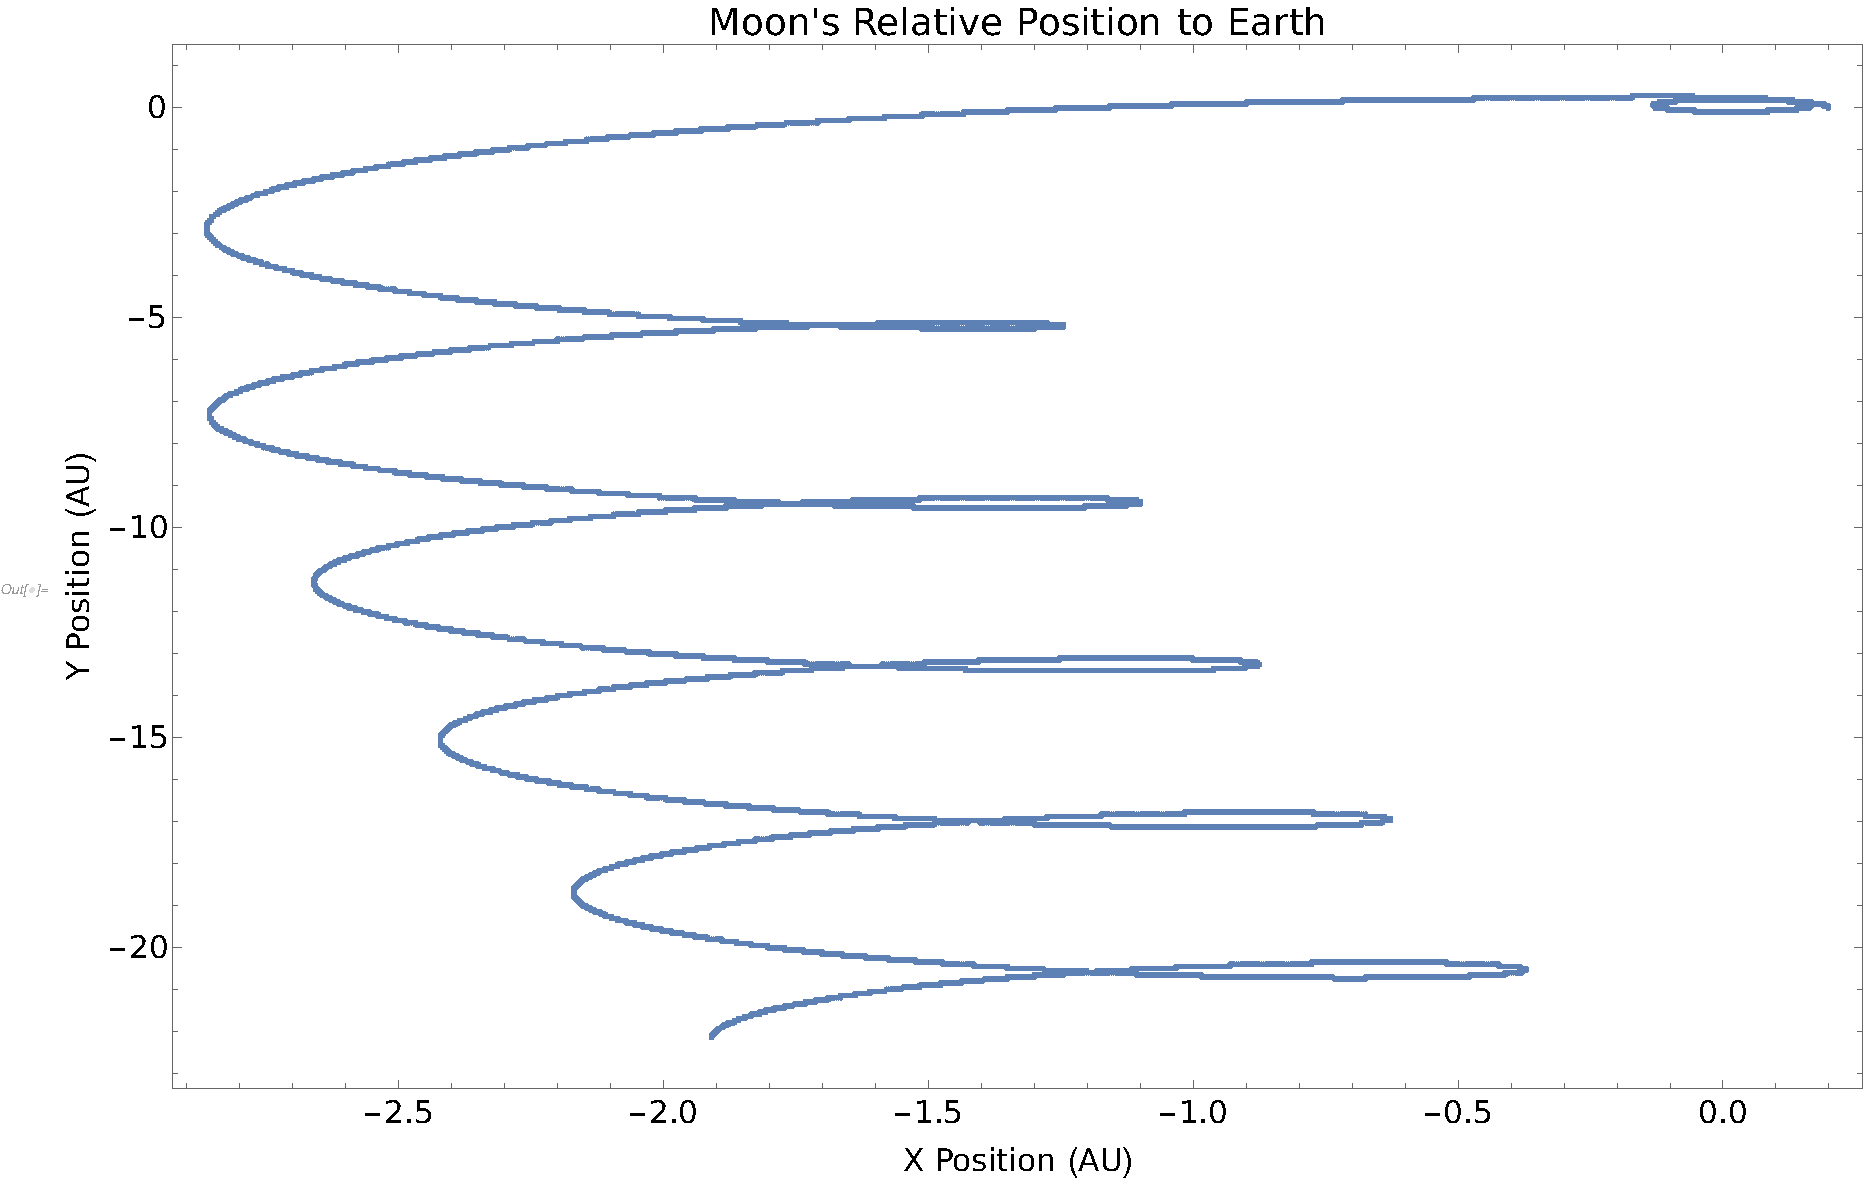
\includegraphics[width=0.5\textwidth]{p1-4b.pdf}
	\end{center}
	\caption{}
\label{fig:qual}
\end{figure}
\FloatBarrier

We can see the ebb and flow of the moons orbit clearly in the Graphic below. There is a gentle trend overall for the moon to drift away from the earth.

\begin{figure}[!htb]
	\begin{center}
		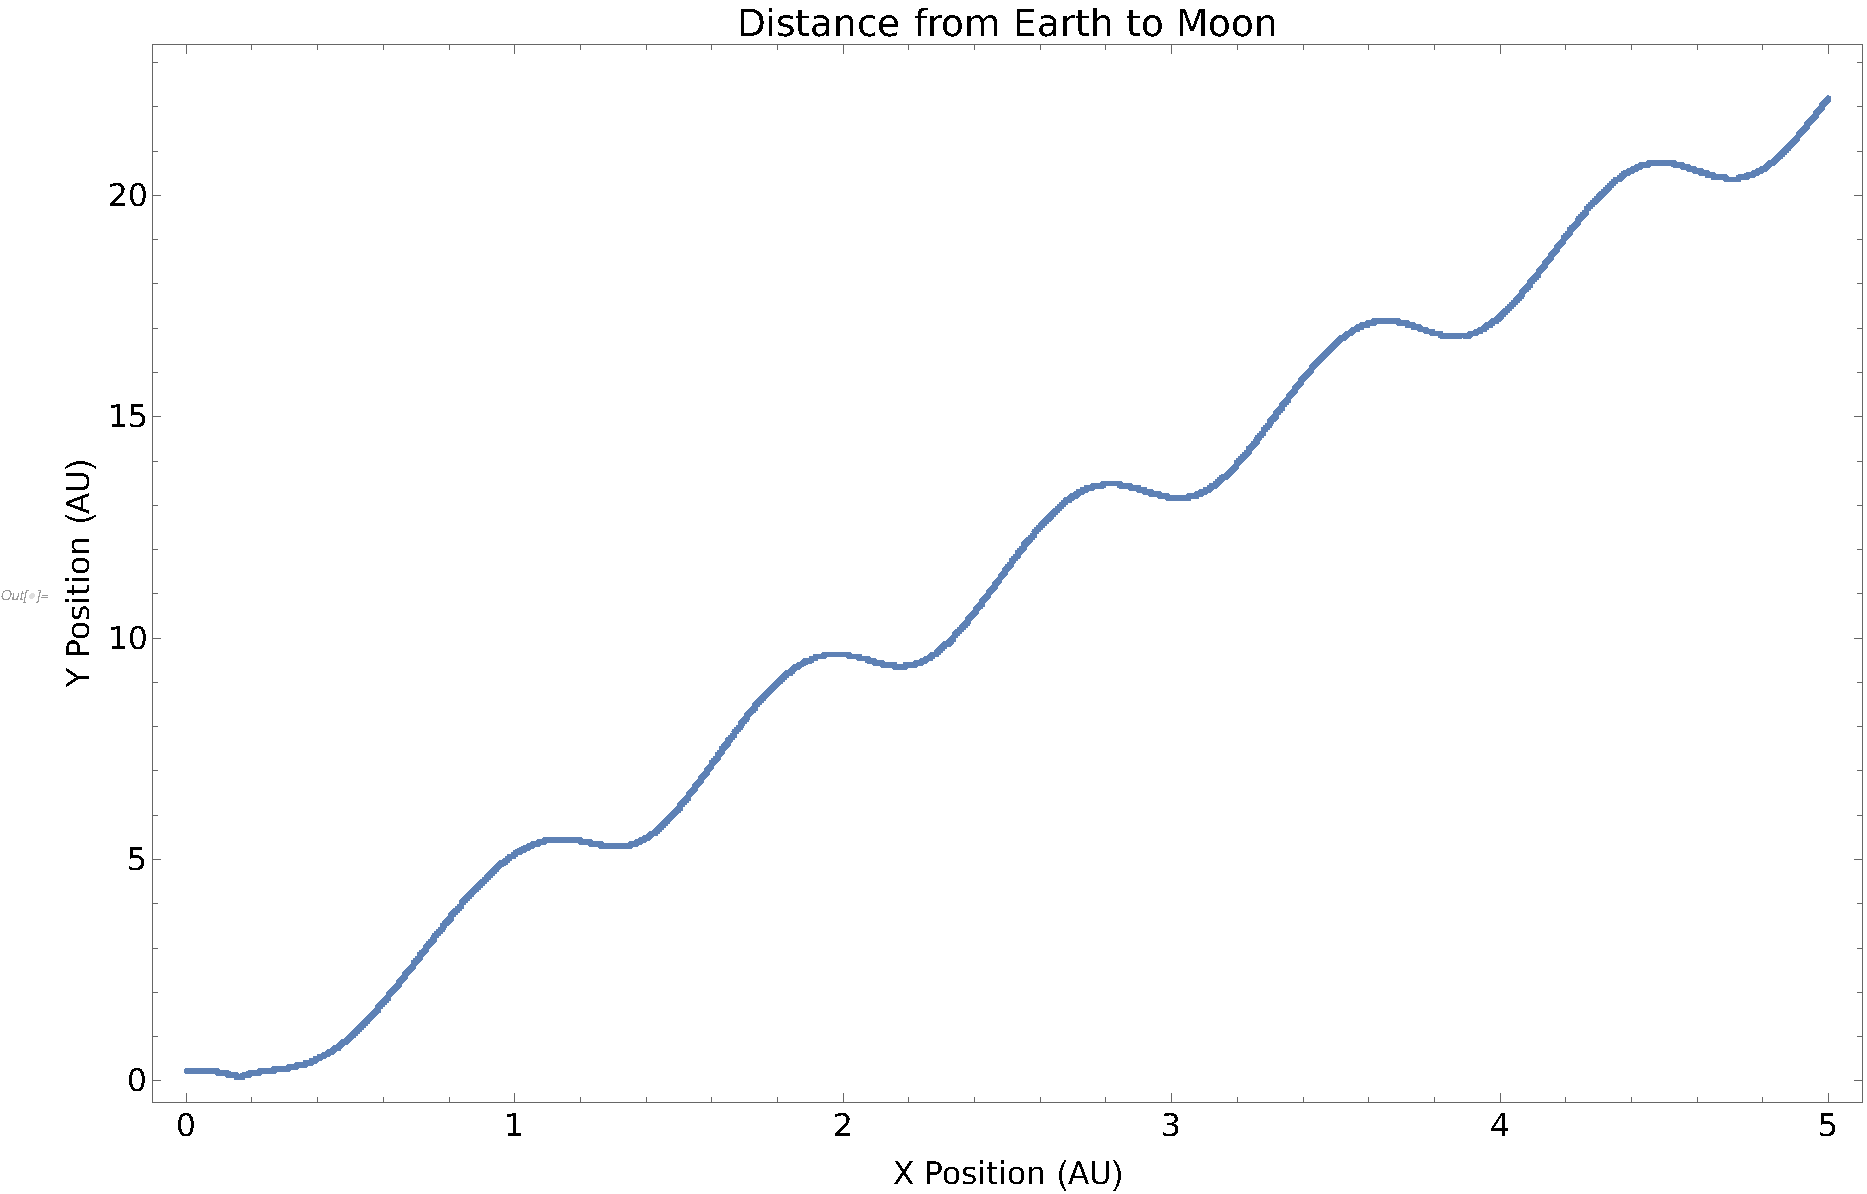
\includegraphics[width=0.5\textwidth]{p1-4c.pdf}
	\end{center}
	\caption{}
\label{fig:qual}
\end{figure}
\FloatBarrier


\begin{figure}[!htb]
	\begin{center}
		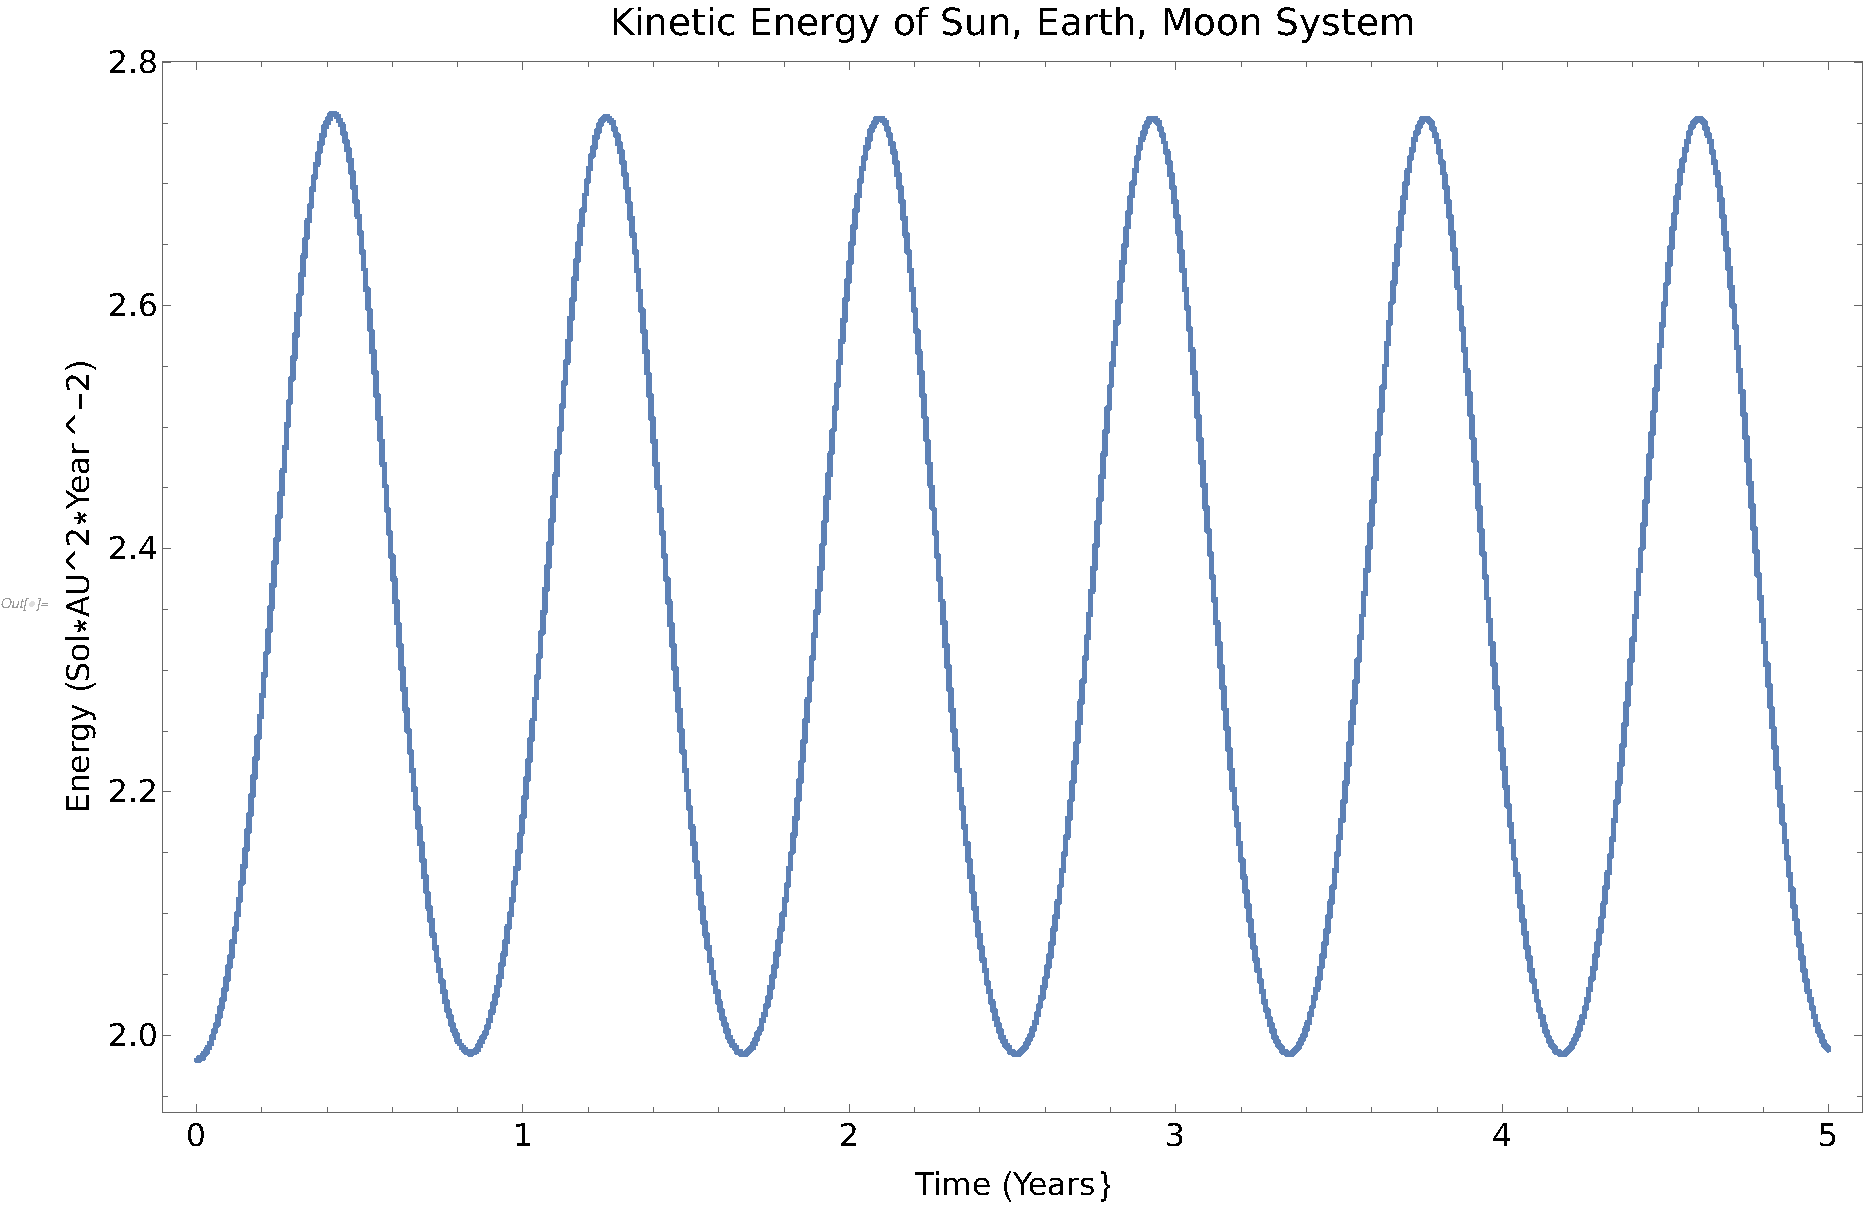
\includegraphics[width=0.5\textwidth]{p1-4d.pdf}
	\end{center}
	\caption{}
\label{fig:qual}
\end{figure}
\FloatBarrier


\begin{figure}[!htb]
	\begin{center}
		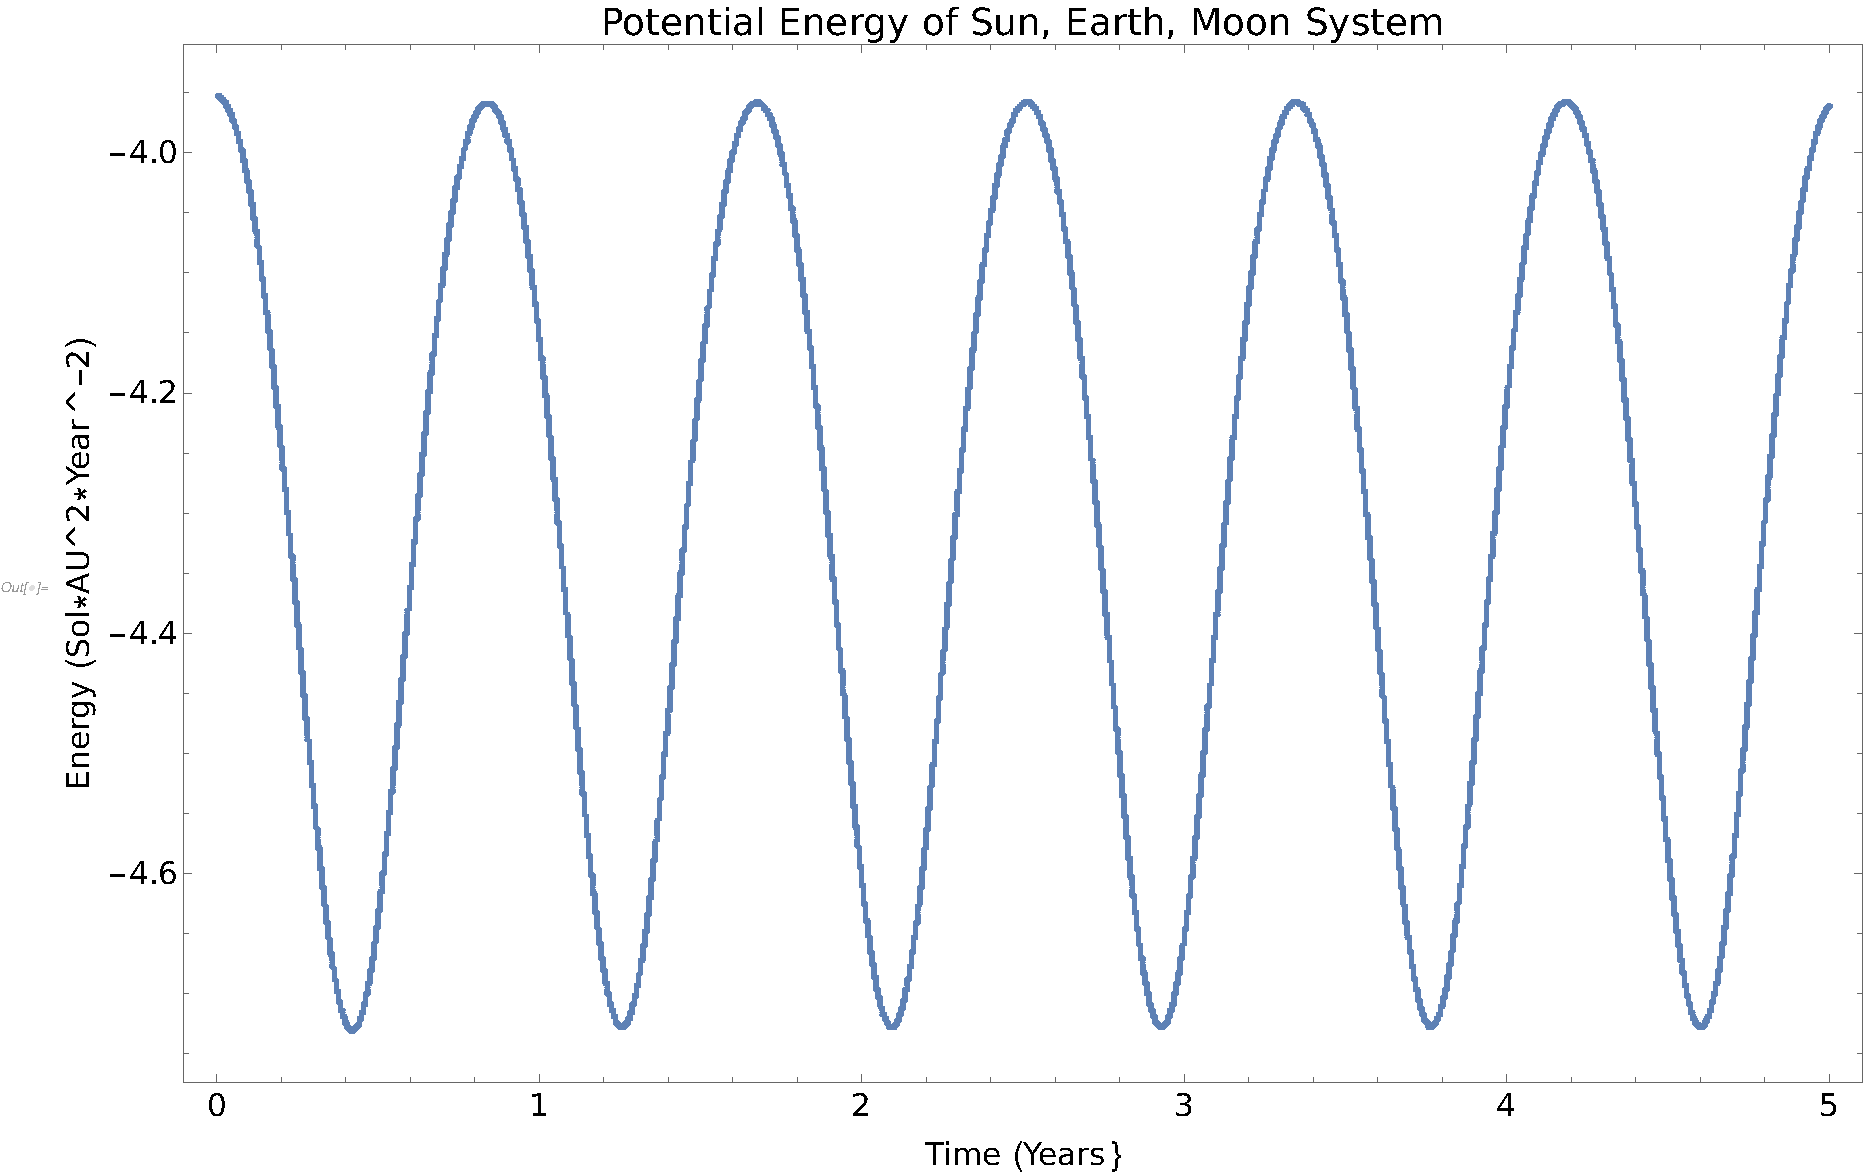
\includegraphics[width=0.5\textwidth]{p1-4e.pdf}
	\end{center}
	\caption{}
\label{fig:qual}
\end{figure}
\FloatBarrier

\begin{figure}[!htb]
	\begin{center}
		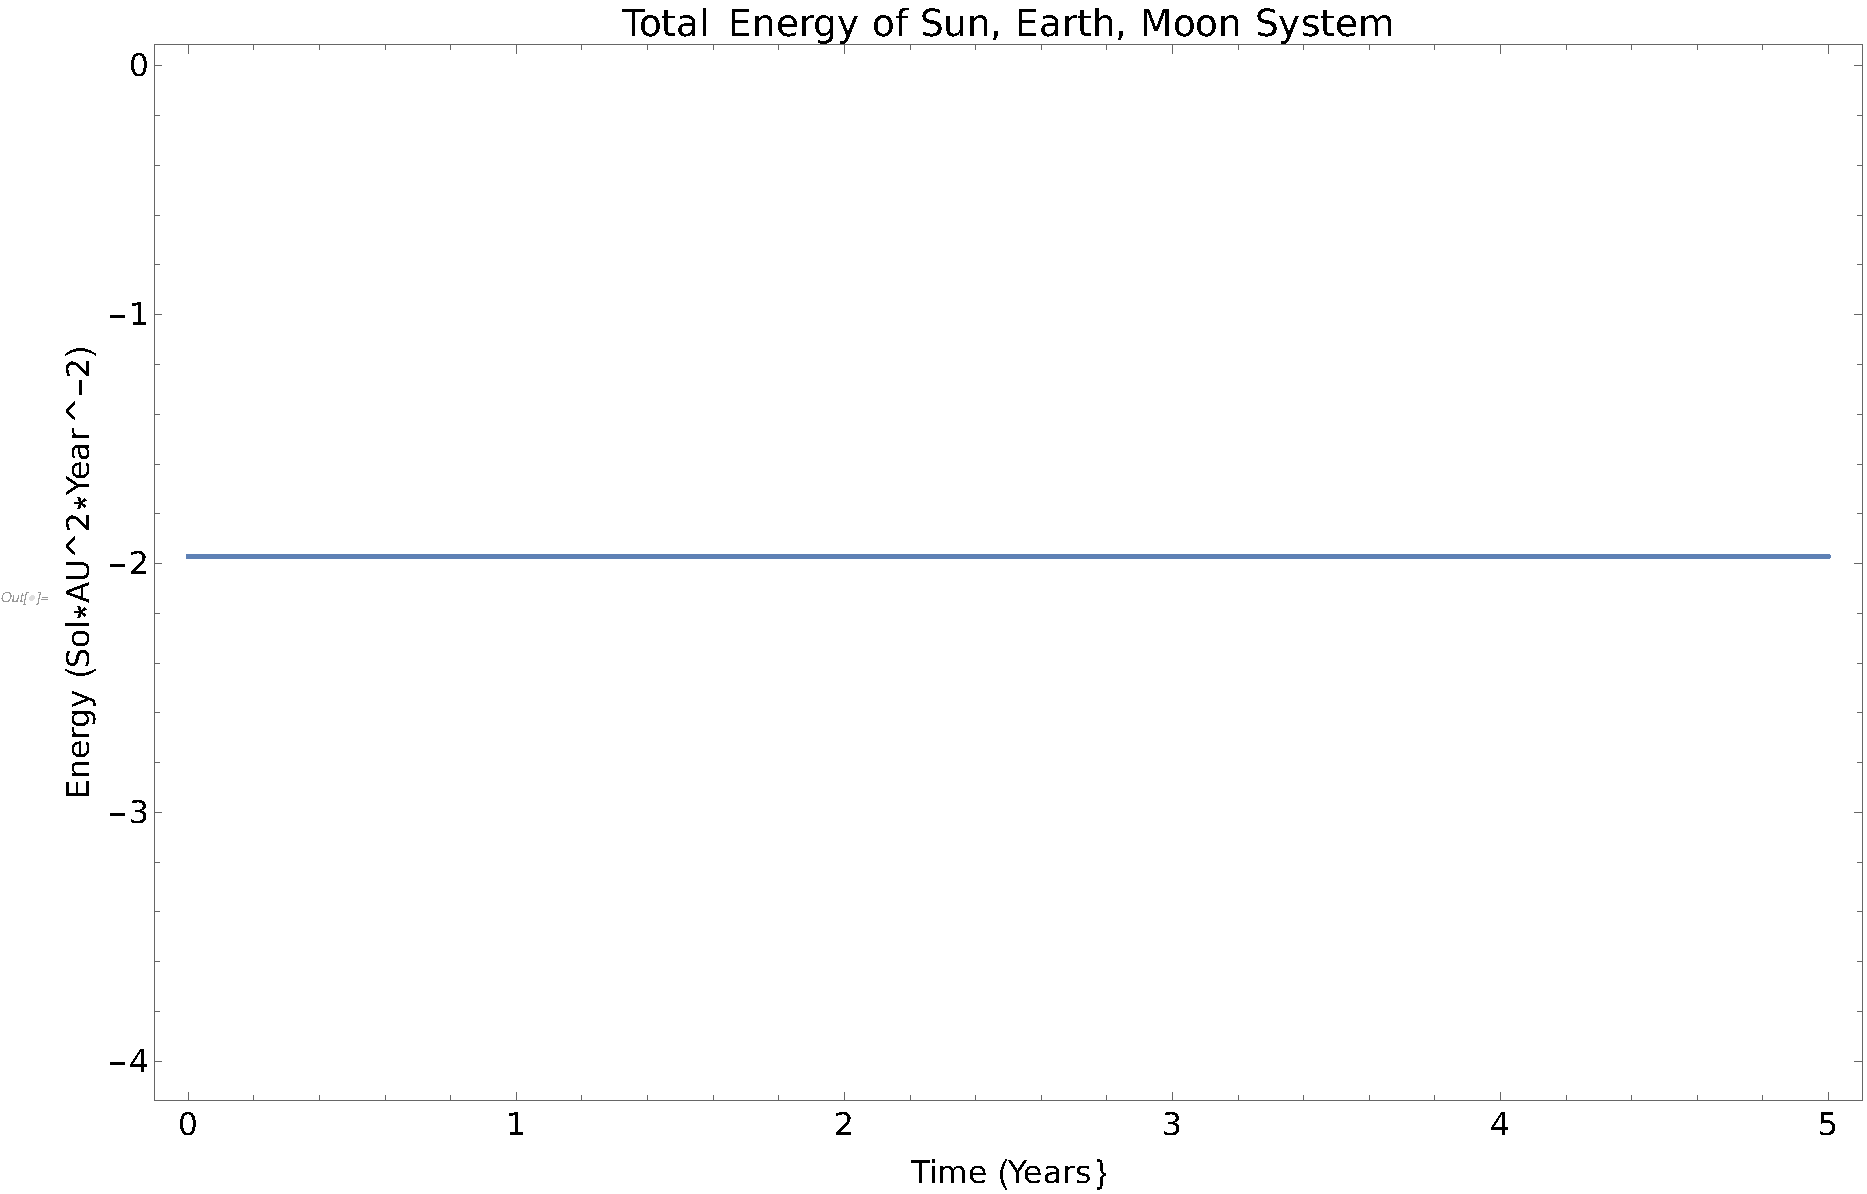
\includegraphics[width=0.5\textwidth]{p1-4f.pdf}
	\end{center}
	\caption{}
\label{fig:qual}
\end{figure}
\FloatBarrier

\subsection{Question 2}

Plotted for $M_1 = M_2 = M_3 = 1, x_1=(0,0), v_1 = (1,-1), x,2 = (1,0), v_2 = (0,6), x_3=(2,0), v_3=(0,6)$ 

Below we see the motion of the 3 bodies relative to the center of mass for the system. It appears very chaotic.

\begin{figure}[!htb]
	\begin{center}
		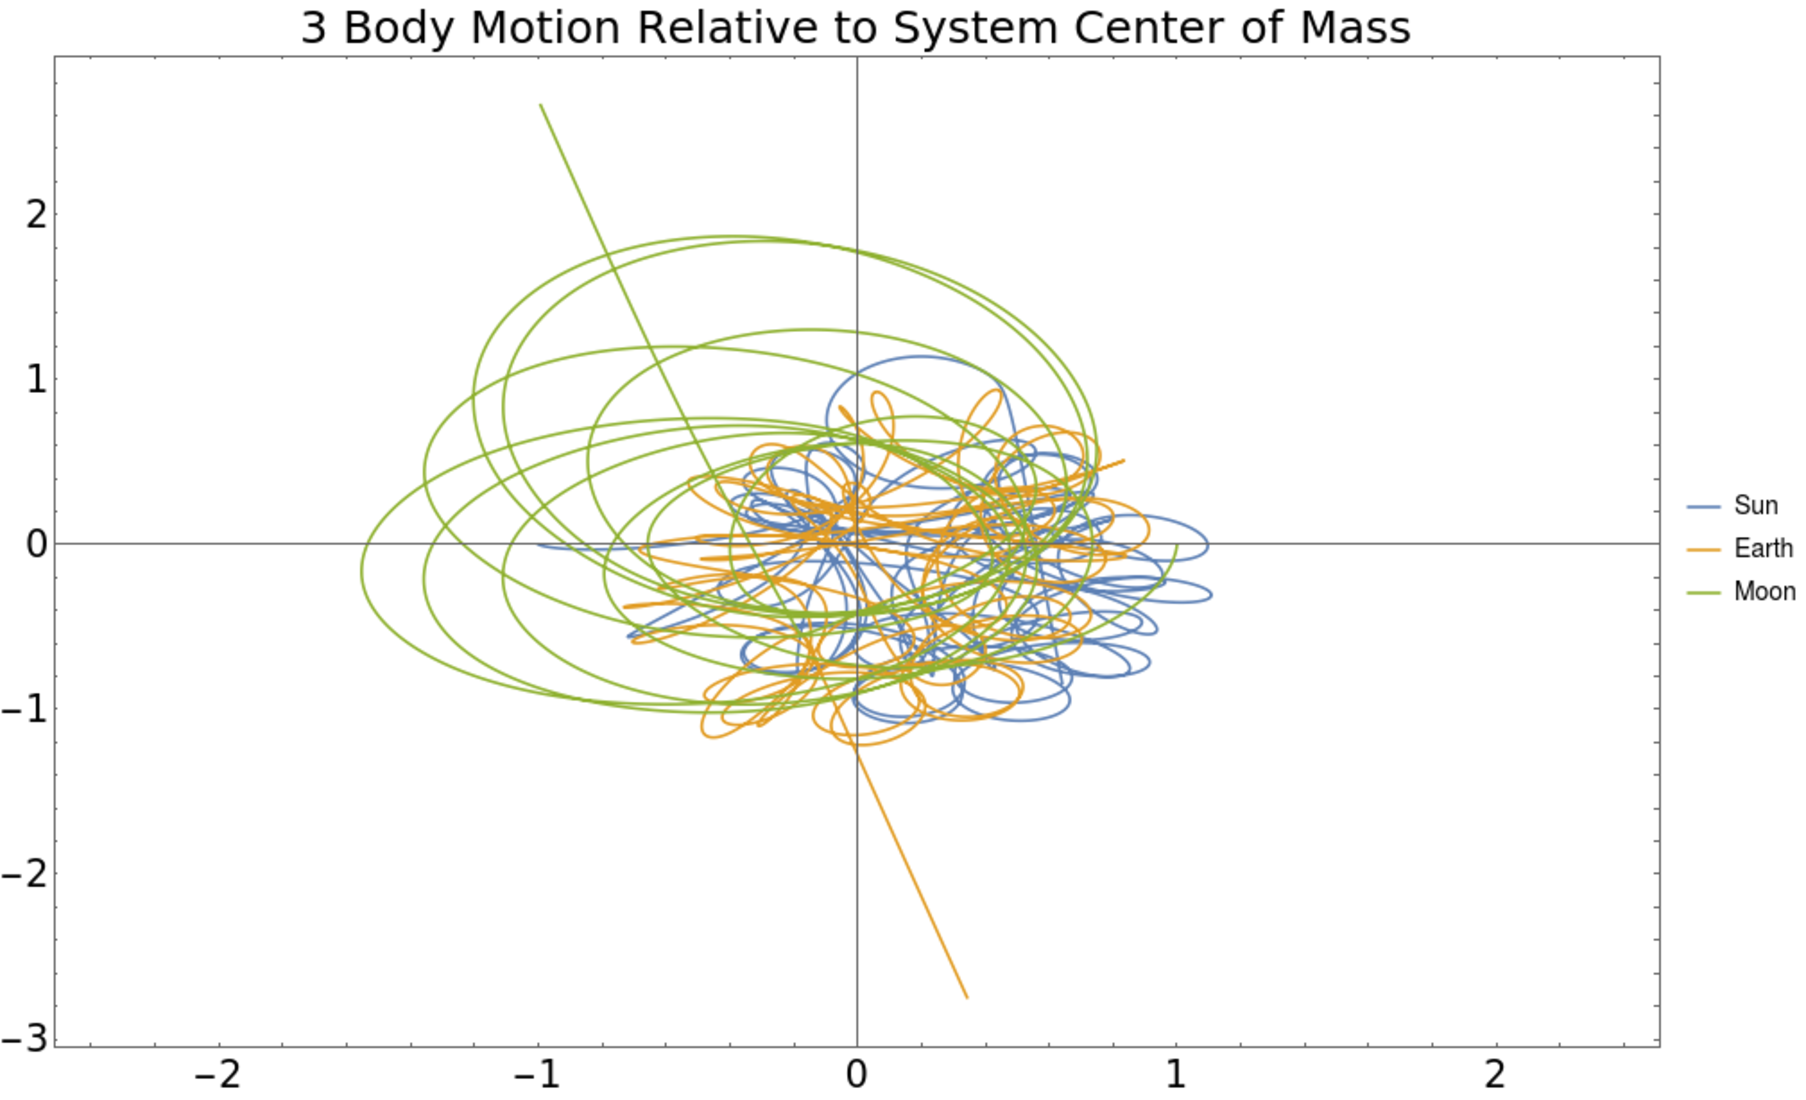
\includegraphics[width=0.5\textwidth]{p2-1a.pdf}
	\end{center}
	\caption{}
\label{fig:qual}
\end{figure}
\FloatBarrier

With out correcting for the drift of the system, the net momentum of the system causes a drift in the positive x and negative y directions.

\begin{figure}[!htb]
	\begin{center}
		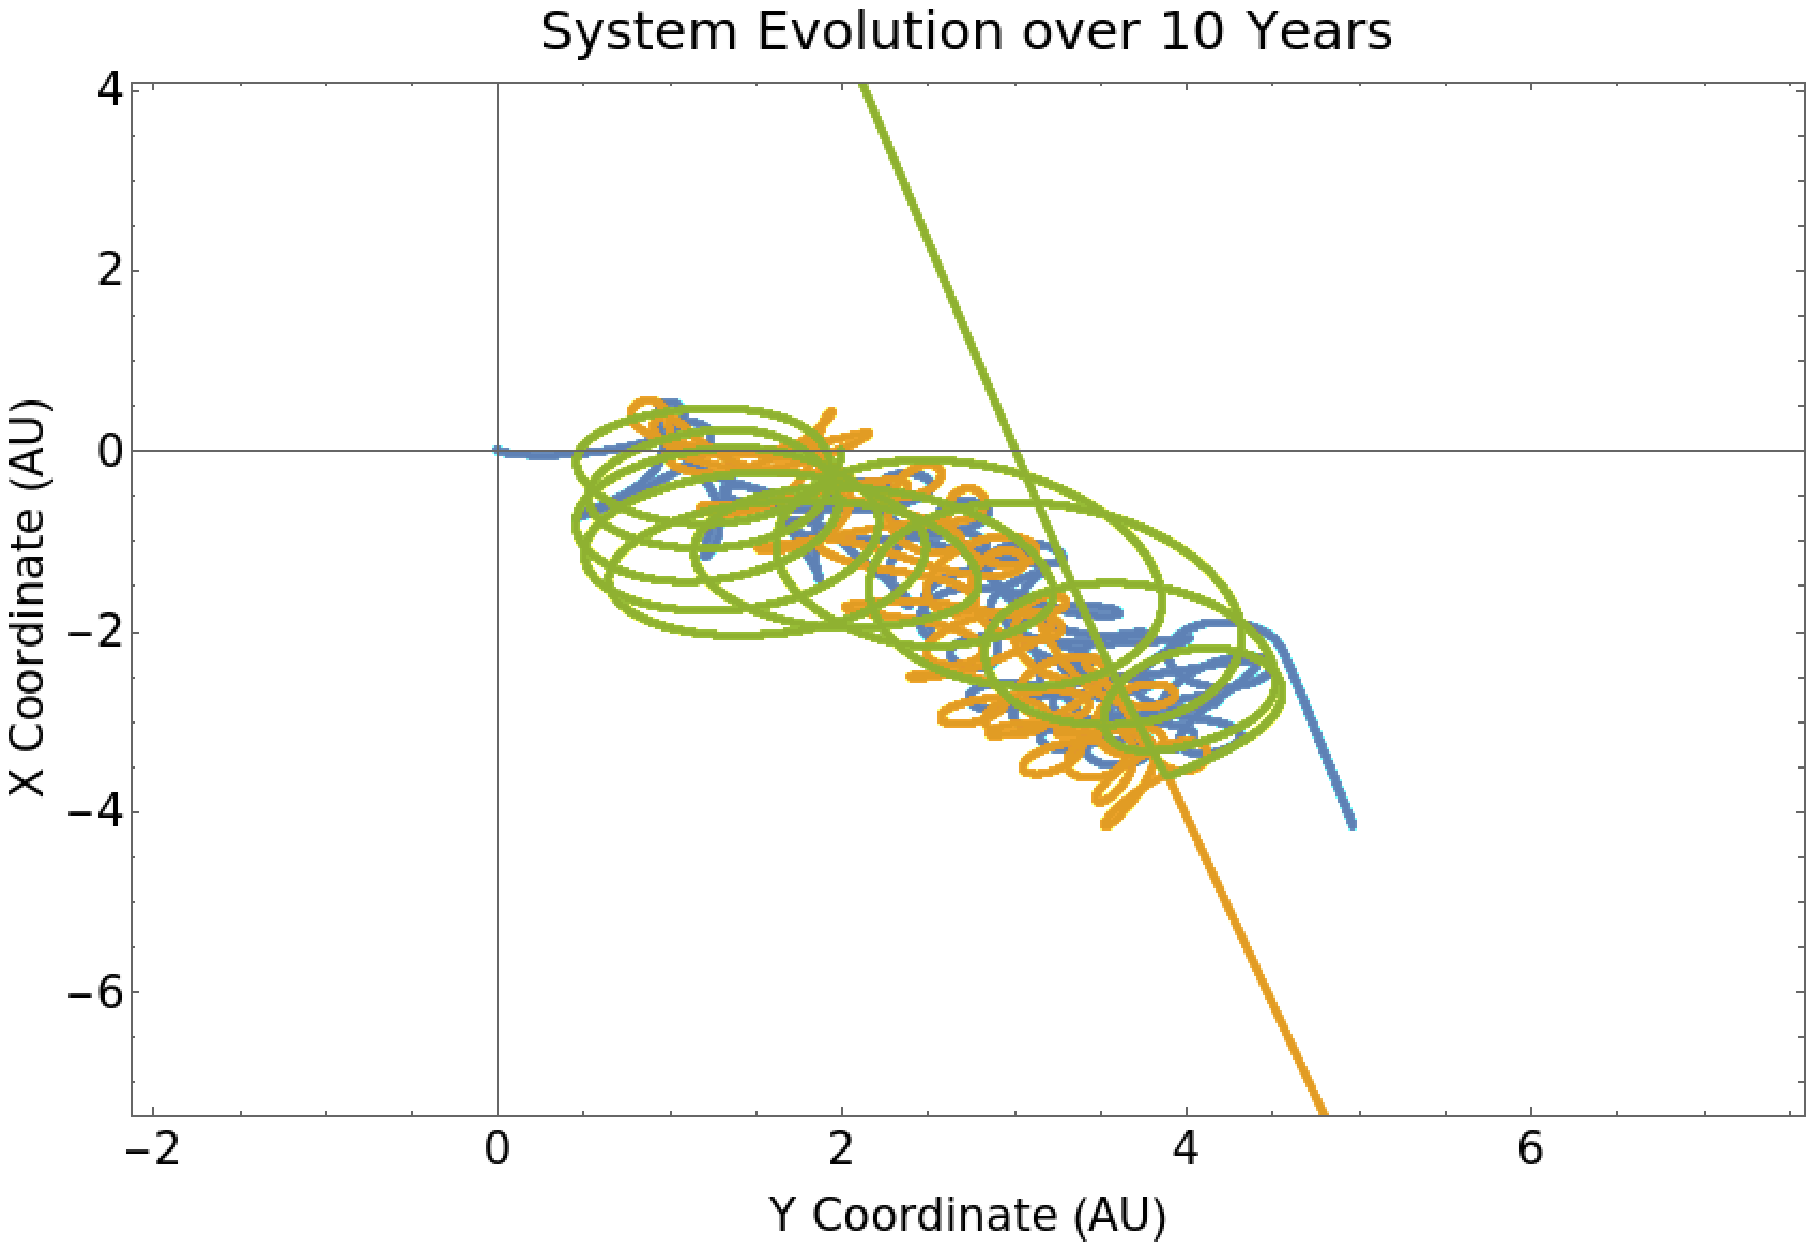
\includegraphics[width=0.5\textwidth]{p2-1b.pdf}
	\end{center}
	\caption{}
\label{fig:qual}
\end{figure}
\FloatBarrier

We can see the ebb and flow of the moons orbit clearly in the Graphic below. There is a gentle trend overall for the moon to drift away from the earth.

\begin{figure}[!htb]
	\begin{center}
		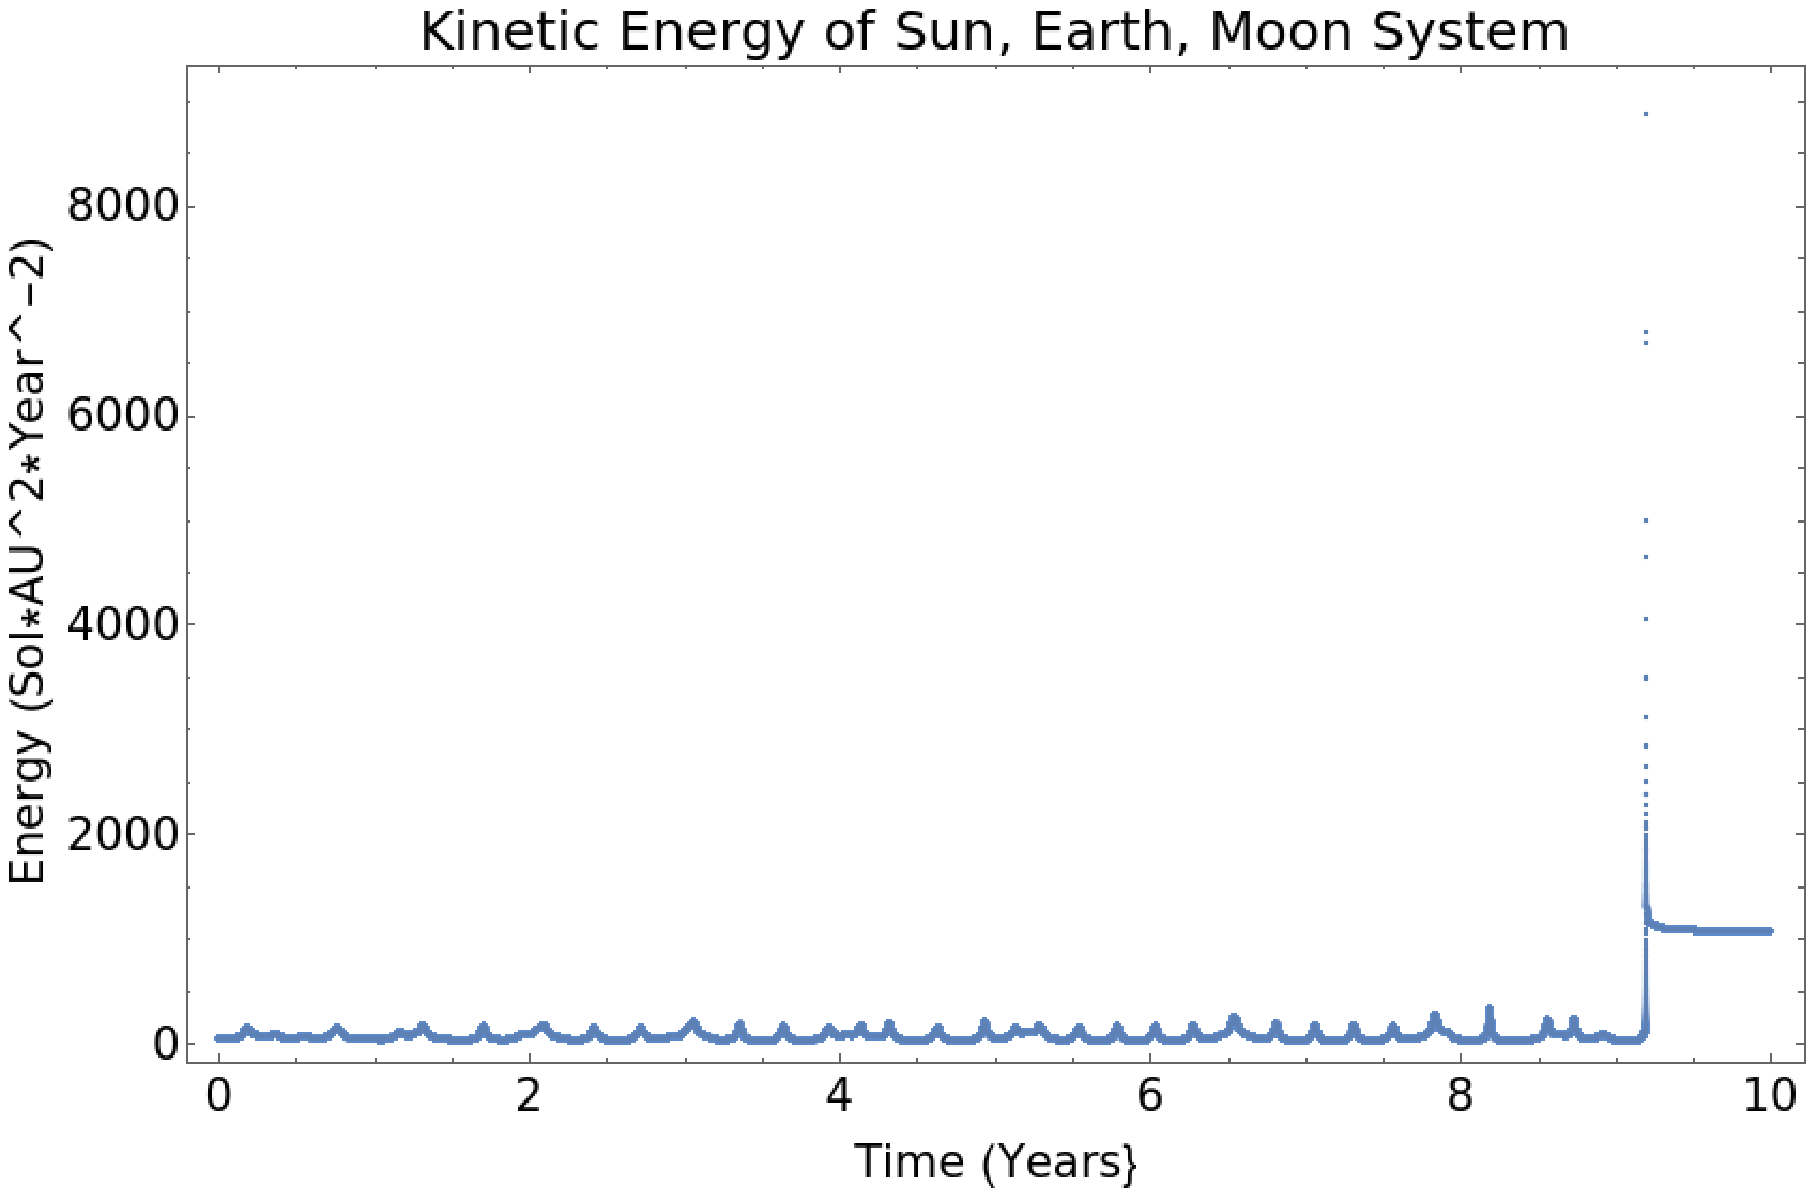
\includegraphics[width=0.5\textwidth]{p2-1c.pdf}
	\end{center}
	\caption{}
\label{fig:qual}
\end{figure}
\FloatBarrier


\begin{figure}[!htb]
	\begin{center}
		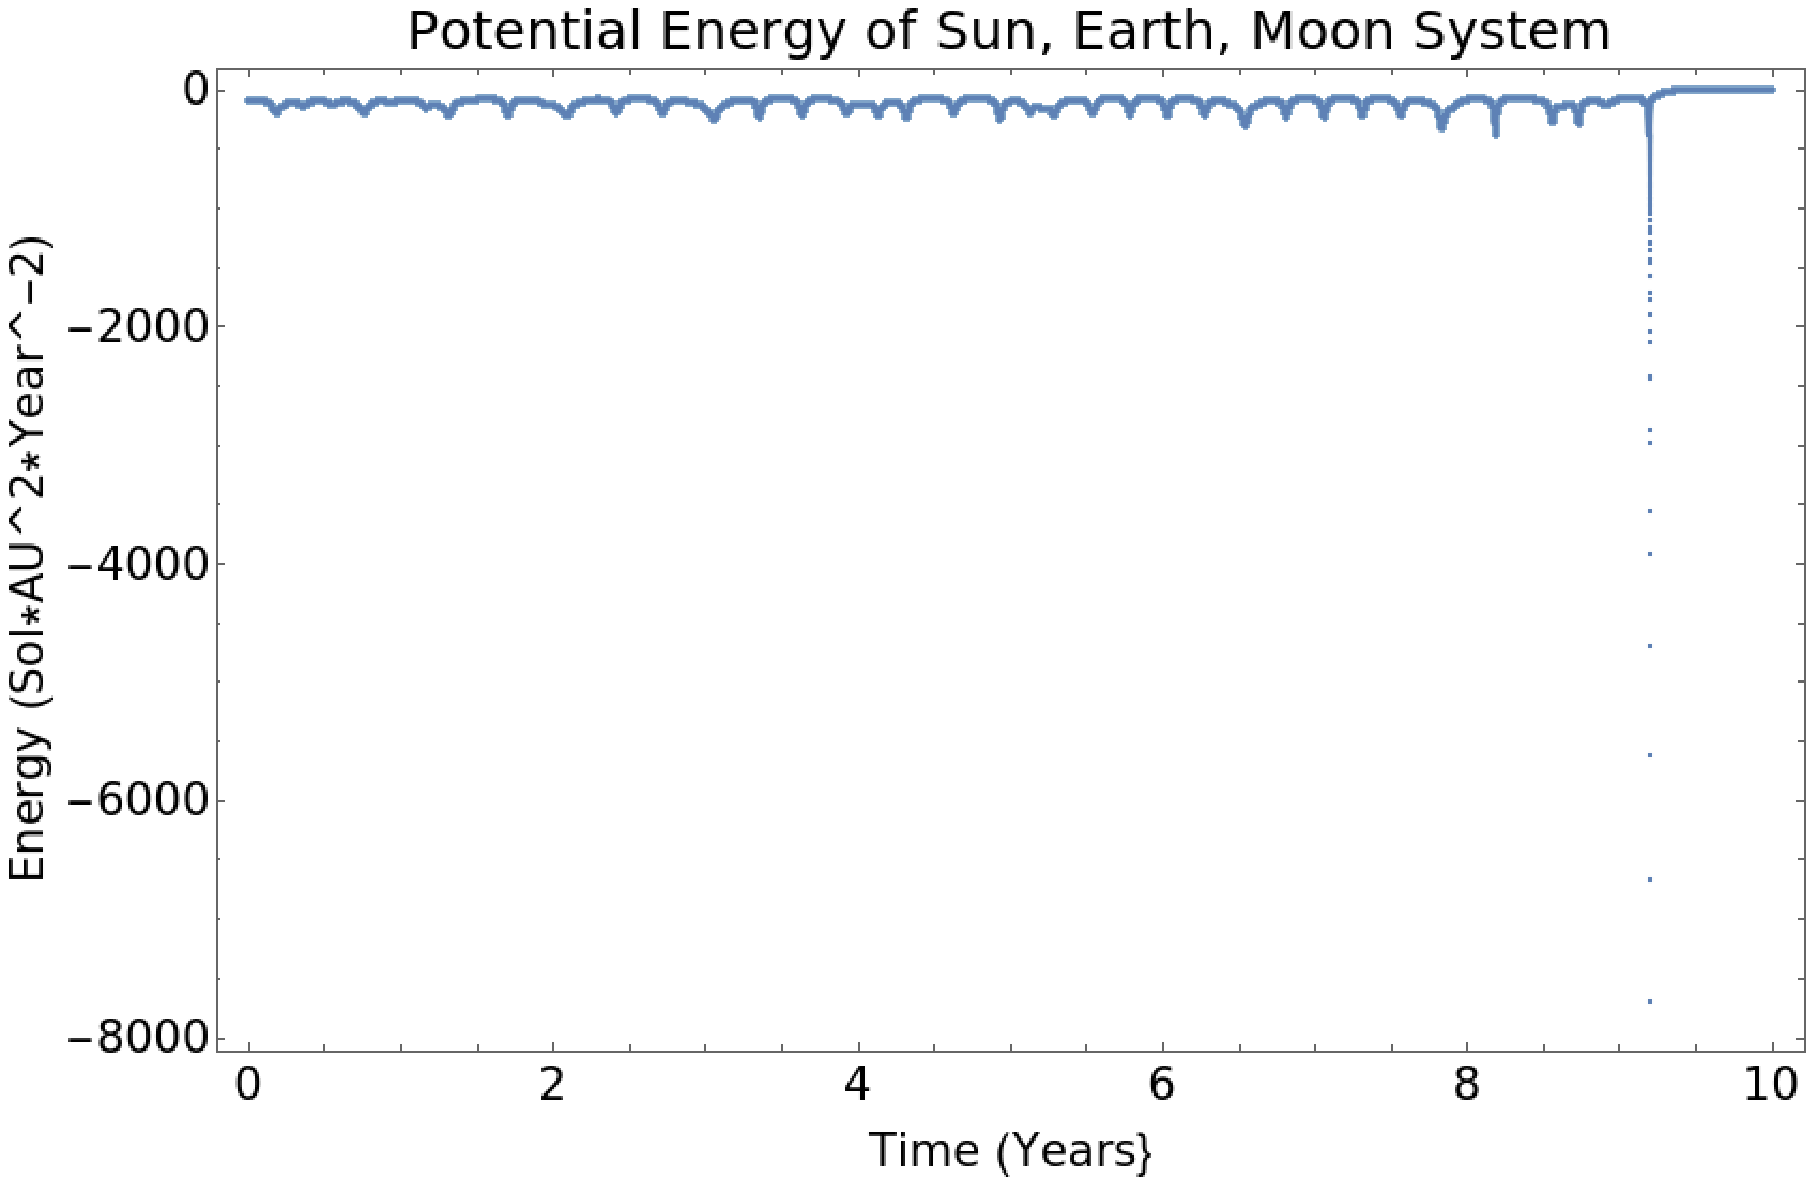
\includegraphics[width=0.5\textwidth]{p2-1d.pdf}
	\end{center}
	\caption{}
\label{fig:qual}
\end{figure}
\FloatBarrier


\begin{figure}[!htb]
	\begin{center}
		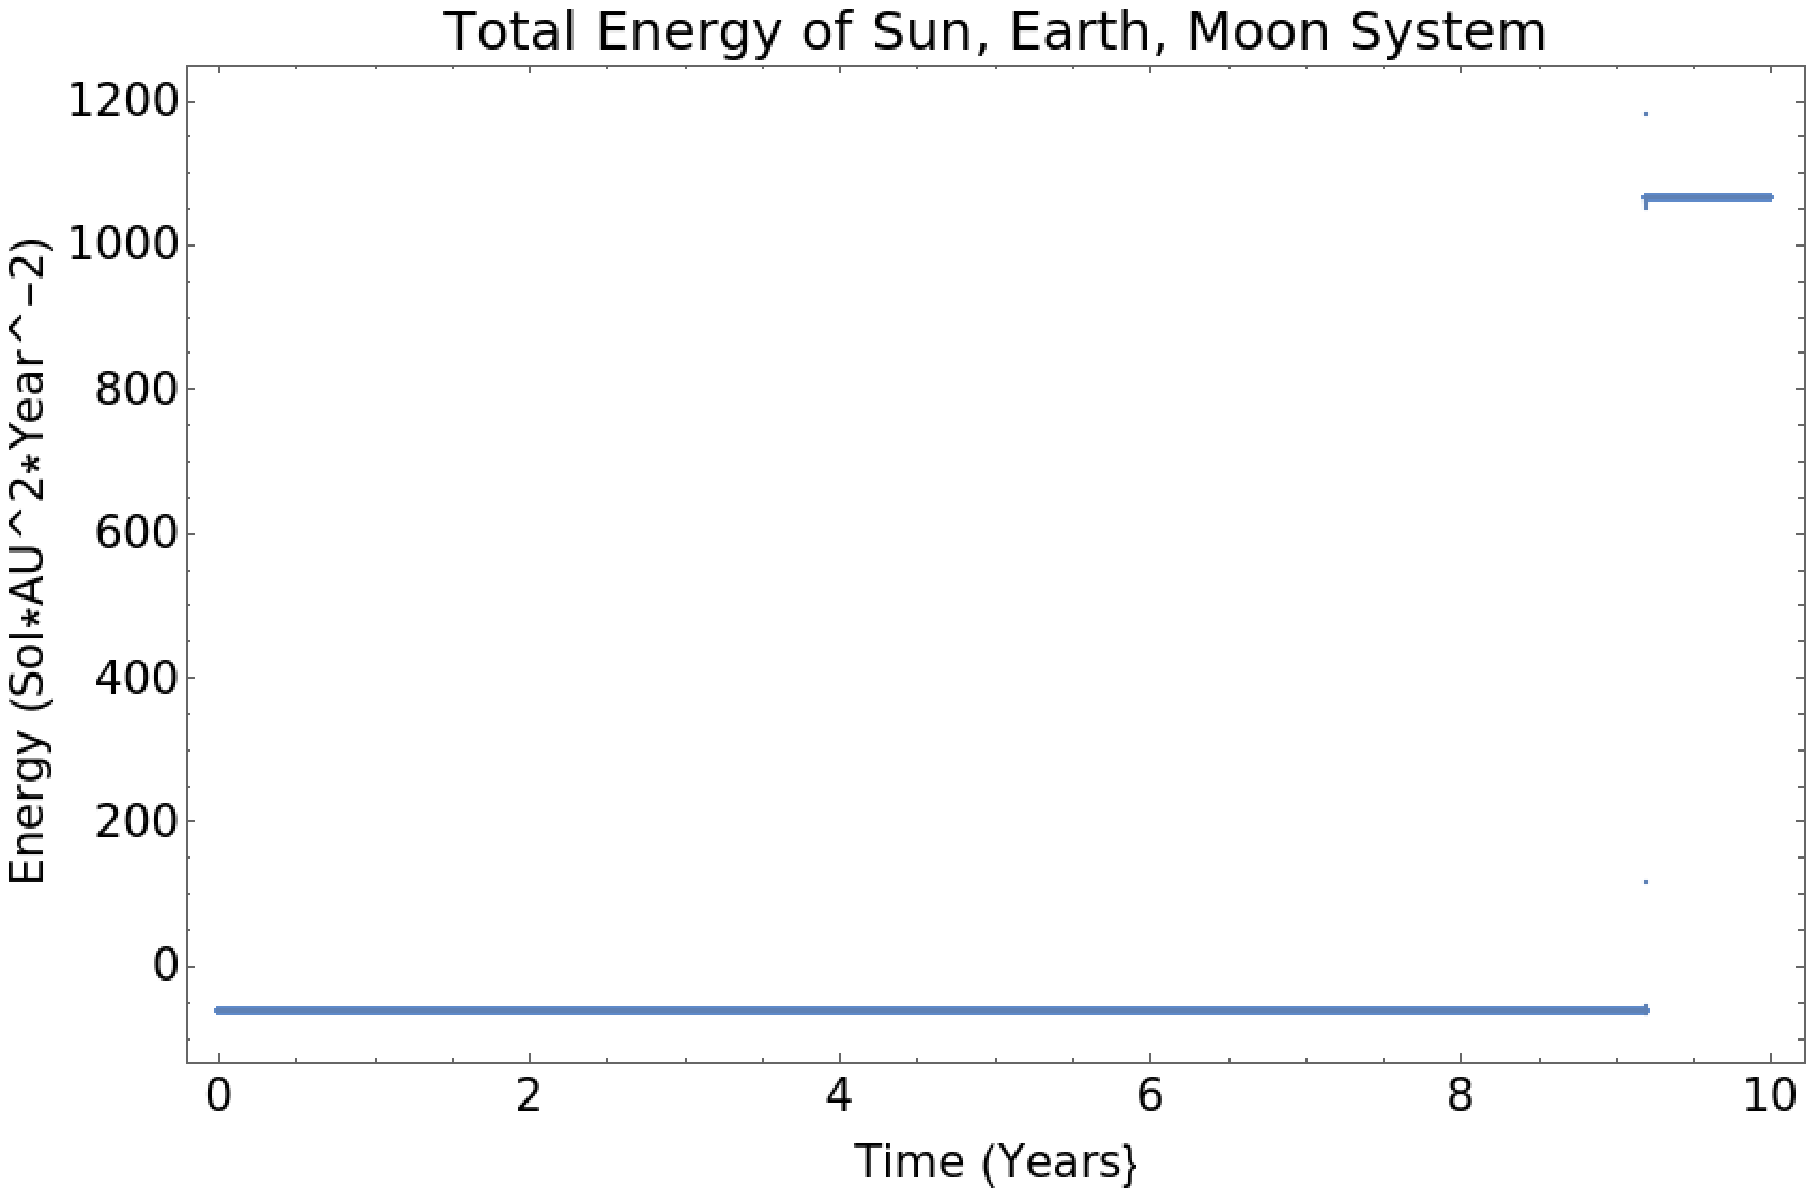
\includegraphics[width=0.5\textwidth]{p2-1e.pdf}
	\end{center}
	\caption{}
\label{fig:qual}
\end{figure}
\FloatBarrier

In the images of energy above, when the bodies get very close, the rate of change of the position and velocity are high enough that the linear approximation over dt is no longer valid. The actual effects of these small separation vectors would most likely caused a collision of the bodies, or of a breakup of one or both of the bodies into smaller chunks. One possible solution is to add collision detection, and allow for a perfectly inelastic collision of the 2 bodies to for 1 large gravitationally bound body, or to implement a "monitoring system" that could dial up or down the time step for systems when 2 bodies get very close.

\subsection{Question 3}
For the $n$-body problem the compute resources required scales as $\mathcal{O}(n^2)$. This is because for each body every other body has to be computed against it. To reduce steps you could compute the effects of $i$ on $j$ at the same time you compute the effects of $j$ on $i$ then you wouldn't need to loop over the full list every time, just loop through  $i>j$. But this doesn't change the  $\mathcal{O}(n^2)$, it would just save some time in the looping. Alternatively, you could threshold each body, and then only compute the effects of nearby objects. To do this you would need to establish a hierarchy of bodies, for example you would compute the effects of the Sun on the Moon, but you could neglect the effects of the Moon on the Sun, while still computing the effect of the Moon on Earth. You could also compute the effects of the CoM on each object. So you would find the CoM for bodies that are relatively close to each other then us the CoM to compute the effects on bodies that are far enough away to treat a cluster of objects as one body.

\subsection{Bonus Question 4}

See the Picture below.

\begin{figure}[!htb]
	\begin{center}
		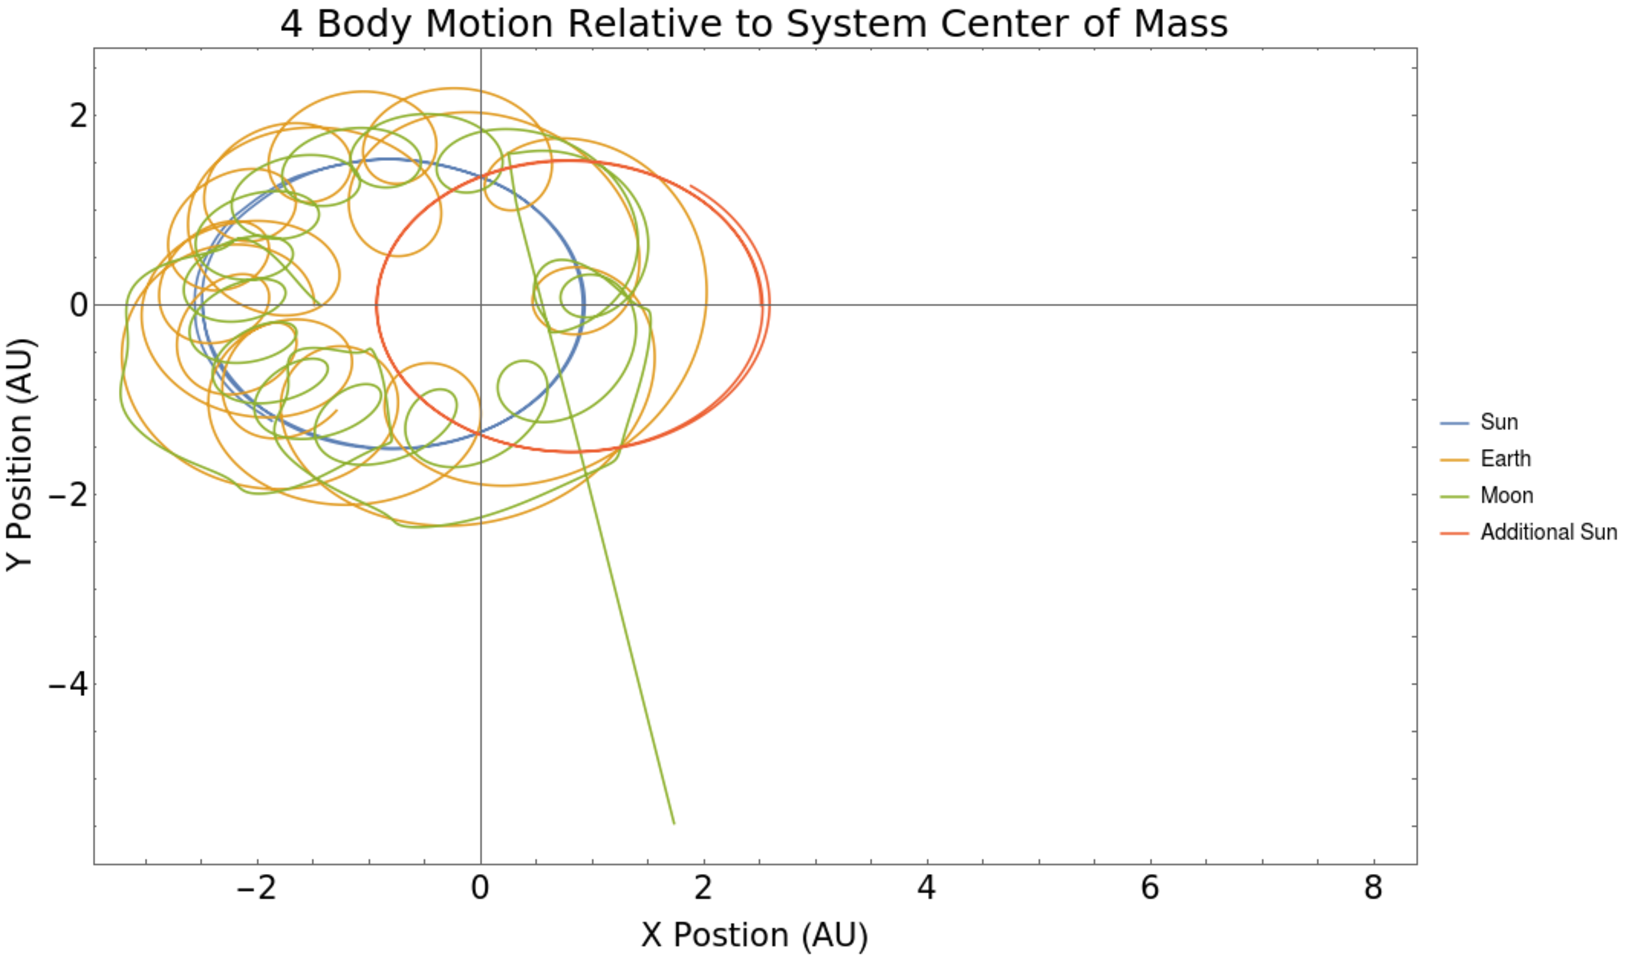
\includegraphics[width=0.5\textwidth]{p4-1a.pdf}
	\end{center}
	\caption{}
\label{fig:qual}
\end{figure}
\FloatBarrier

Here we have created a binary star system with 2 one Sol mass objects. 

Around one of the Stars, a Earth/Moon system is put into orbit. The orbits of the Planet/Moon system is complicated immensely by the existence of the second star. Because of this the orbits they follow are highly irregular and eventually the Moon is ejected from the system when it ventures too close to its host planet.

The Dominant Forces are the 2 main stars, while the Planets gravity is subdominant on the moon.


\section{Conclusions}

This Project was rather neat. One tweak I made to the code was to ignore interactions between objects if the length of the separation vector was zero. This prevented a significant number of \tttext{-nan} errors, this was especially useful when working with 2 body systems to suppress errors caused by nonexistent bodies that had mass of zero. 

\end{document}
